\section{Arts\-Engine Class Reference}
\label{classArtsEngine}\index{ArtsEngine@{ArtsEngine}}
{\tt \#include $<$artsengine.h$>$}

Inheritance diagram for Arts\-Engine:\begin{figure}[H]
\begin{center}
\leavevmode
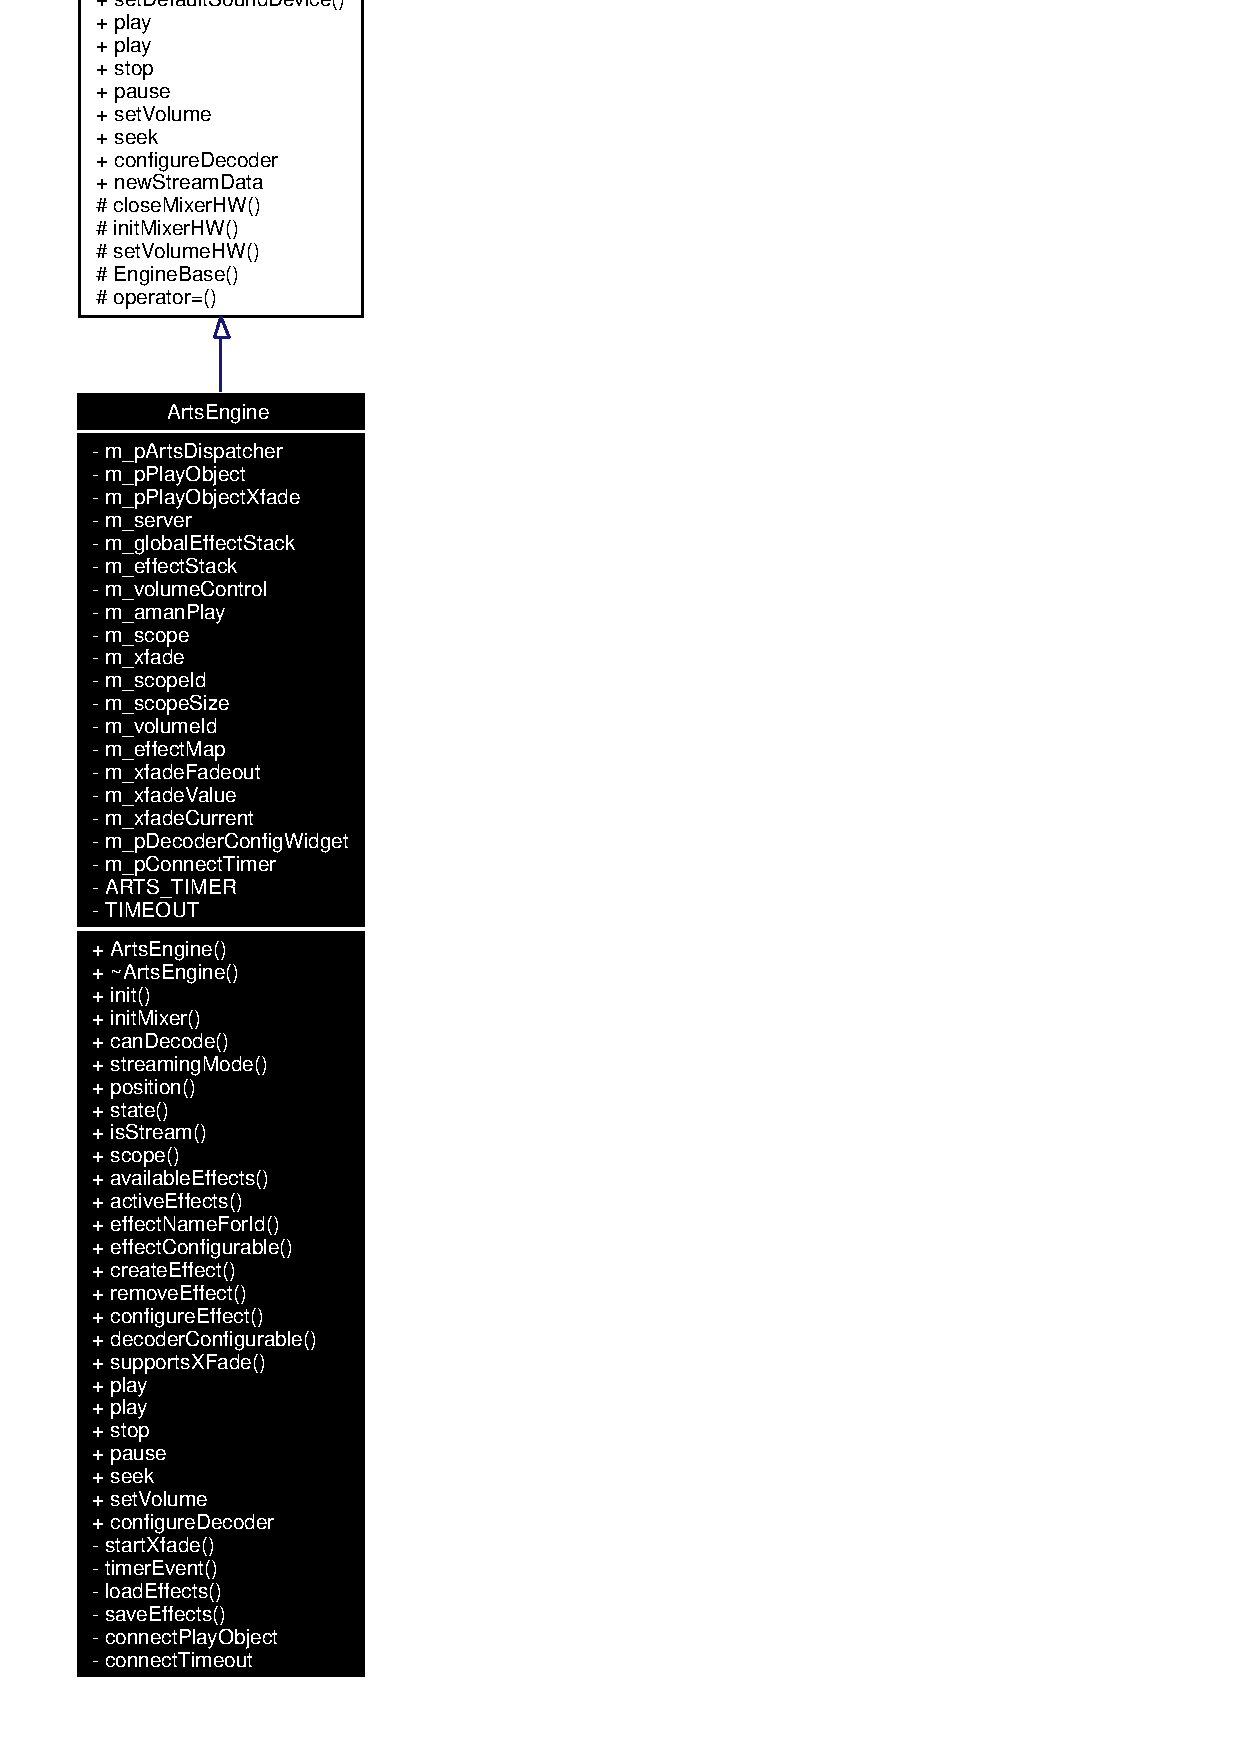
\includegraphics[width=88pt]{classArtsEngine__inherit__graph}
\end{center}
\end{figure}
Collaboration diagram for Arts\-Engine:\begin{figure}[H]
\begin{center}
\leavevmode
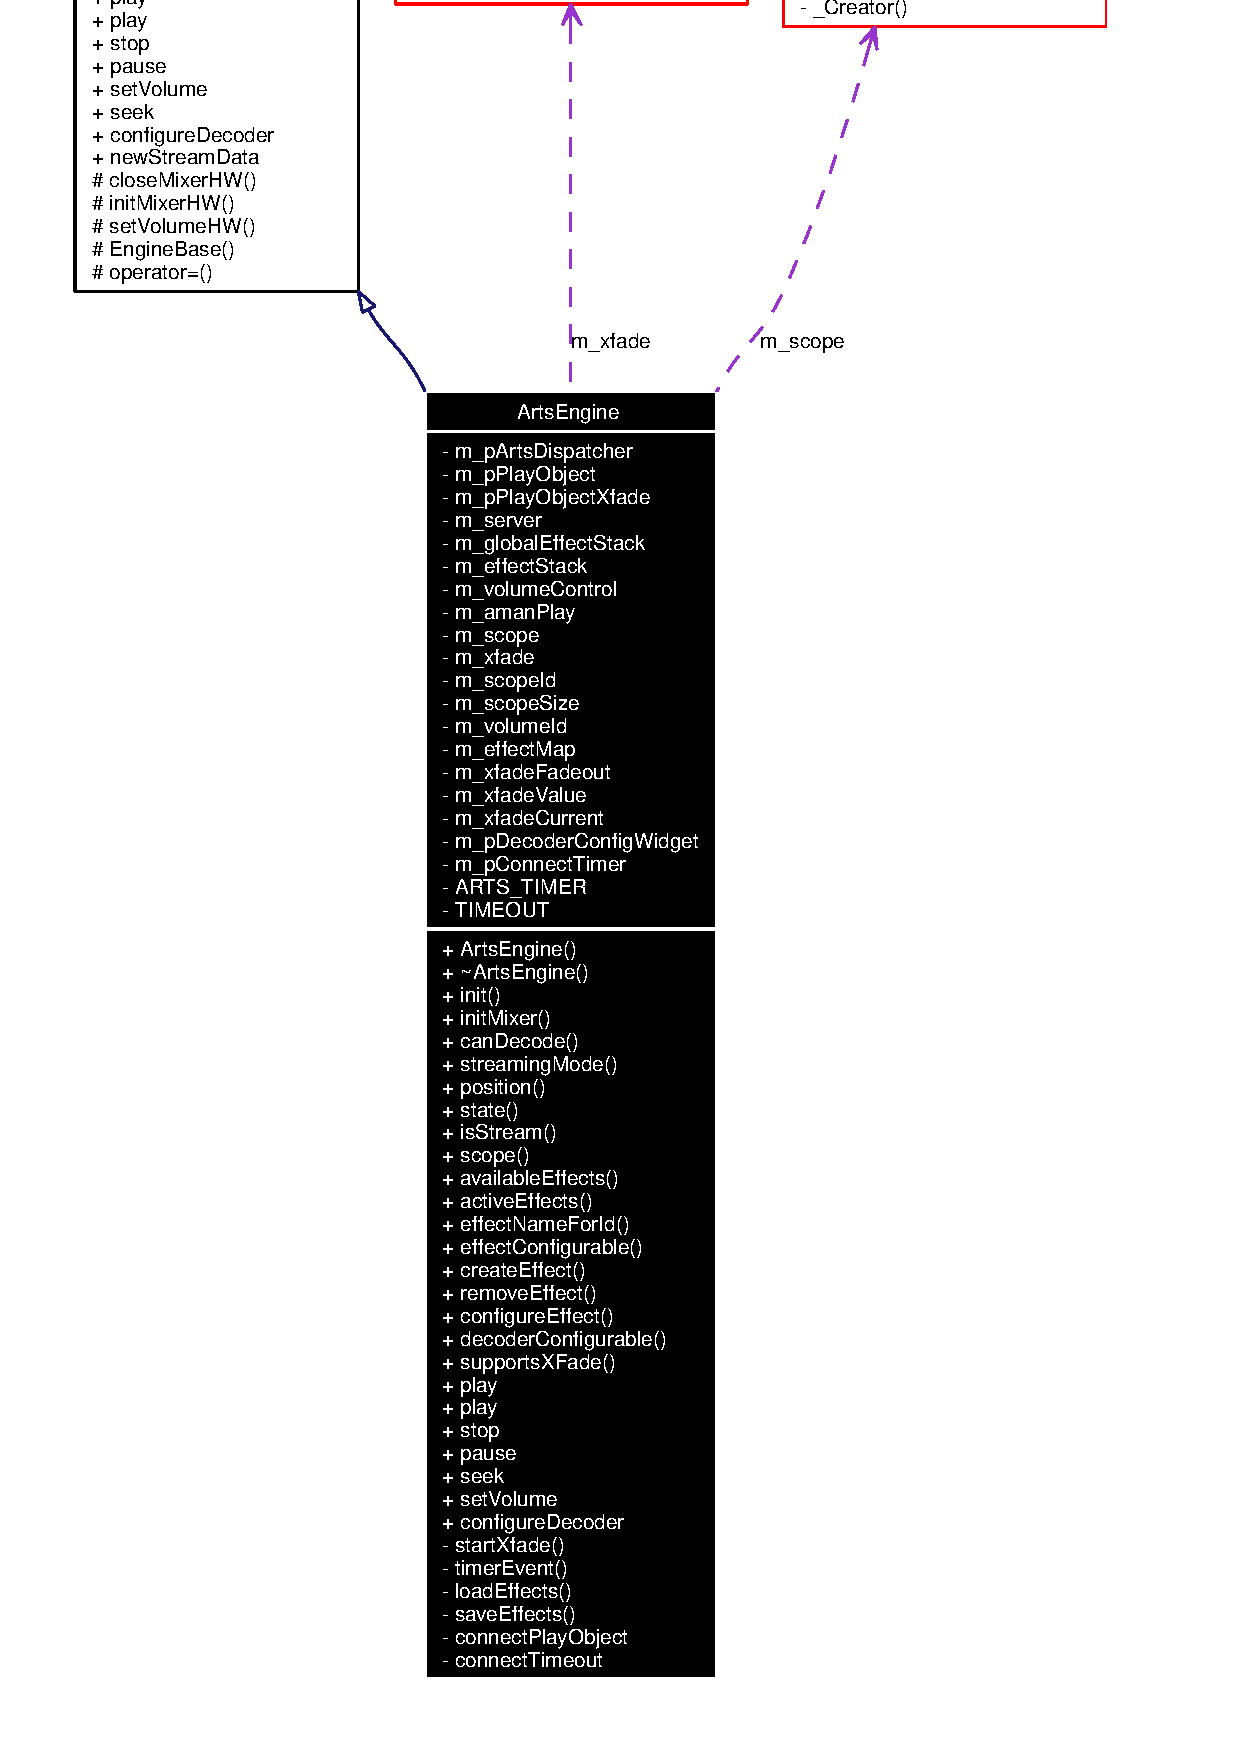
\includegraphics[width=265pt]{classArtsEngine__coll__graph}
\end{center}
\end{figure}
\subsection*{Public Types}
\begin{CompactItemize}
\item 
enum {\bf Engine\-State} \{ {\bf Empty}, 
{\bf Idle}, 
{\bf Playing}, 
{\bf Paused}
 \}
\item 
enum {\bf Streaming\-Mode} \{ {\bf Socket}, 
{\bf Signal}, 
{\bf No\-Streaming}
 \}
\end{CompactItemize}
\subsection*{Public Slots}
\begin{CompactItemize}
\item 
void {\bf play} (const KURL \&)
\item 
void {\bf play} ()
\item 
void {\bf stop} ()
\item 
void {\bf pause} ()
\item 
void {\bf seek} (long ms)
\item 
void {\bf set\-Volume} (int percent)
\item 
void {\bf configure\-Decoder} ()
\item 
virtual void {\bf new\-Stream\-Data} (char $\ast$, int)
\end{CompactItemize}
\subsection*{Signals}
\begin{CompactItemize}
\item 
void {\bf end\-Of\-Track} ()
\item 
void {\bf stopped} ()
\end{CompactItemize}
\subsection*{Public Member Functions}
\begin{CompactItemize}
\item 
{\bf Arts\-Engine} ()
\item 
{\bf $\sim$Arts\-Engine} ()
\item 
void {\bf init} (bool \&restart, int scope\-Size, bool restore\-Effects)
\item 
bool {\bf init\-Mixer} (bool hardware)
\item 
bool {\bf can\-Decode} (const KURL \&url, mode\_\-t mode, mode\_\-t permissions)
\item 
{\bf Streaming\-Mode} {\bf streaming\-Mode} ()
\item 
long {\bf position} () const 
\item 
{\bf Engine\-Base::Engine\-State} {\bf state} () const 
\item 
bool {\bf is\-Stream} () const 
\item 
std::vector$<$ float $>$ $\ast$ {\bf scope} ()
\item 
QString\-List {\bf available\-Effects} () const 
\item 
std::vector$<$ long $>$ {\bf active\-Effects} () const 
\item 
QString {\bf effect\-Name\-For\-Id} (long id) const 
\item 
bool {\bf effect\-Configurable} (long id) const 
\item 
long {\bf create\-Effect} (const QString \&name)
\item 
void {\bf remove\-Effect} (long id)
\item 
void {\bf configure\-Effect} (long id)
\item 
bool {\bf decoder\-Configurable} ()
\item 
bool {\bf supports\-XFade} () const 
\item 
virtual QString\-List {\bf get\-Outputs\-List} ()
\item 
bool {\bf loaded} ()
\item 
int {\bf volume} () const 
\item 
bool {\bf is\-Mixer\-Hardware} () const 
\item 
void {\bf set\-Restore\-Effects} (bool yes)
\item 
virtual bool {\bf decoder\-Configurable} () const 
\item 
virtual void {\bf set\-Xfade\-Length} (int ms)
\item 
virtual void {\bf set\-Sound\-Output} (const QString \&output)
\item 
virtual void {\bf set\-Sound\-Device} (const QString \&device)
\item 
virtual void {\bf set\-Default\-Sound\-Device} (bool is\-Default)
\end{CompactItemize}
\subsection*{Protected Member Functions}
\begin{CompactItemize}
\item 
void {\bf close\-Mixer\-HW} ()
\item 
bool {\bf init\-Mixer\-HW} ()
\item 
void {\bf set\-Volume\-HW} (int percent)
\end{CompactItemize}
\subsection*{Protected Attributes}
\begin{CompactItemize}
\item 
int {\bf m\_\-mixer\-HW}
\item 
int {\bf m\_\-volume}
\item 
int {\bf m\_\-xfade\-Length}
\item 
bool {\bf m\_\-restore\-Effects}
\item 
QString {\bf m\_\-sound\-Output}
\item 
QString {\bf m\_\-sound\-Device}
\item 
bool {\bf m\_\-default\-Sound\-Device}
\end{CompactItemize}
\subsection*{Private Slots}
\begin{CompactItemize}
\item 
void {\bf connect\-Play\-Object} ()
\item 
void {\bf connect\-Timeout} ()
\end{CompactItemize}
\subsection*{Private Member Functions}
\begin{CompactItemize}
\item 
void {\bf start\-Xfade} ()
\item 
void {\bf timer\-Event} (QTimer\-Event $\ast$)
\item 
void {\bf load\-Effects} ()
\item 
void {\bf save\-Effects} ()
\end{CompactItemize}
\subsection*{Private Attributes}
\begin{CompactItemize}
\item 
KArts\-Dispatcher $\ast$ {\bf m\_\-p\-Arts\-Dispatcher}
\item 
KDE::Play\-Object $\ast$ {\bf m\_\-p\-Play\-Object}
\item 
KDE::Play\-Object $\ast$ {\bf m\_\-p\-Play\-Object\-Xfade}
\item 
Arts::Sound\-Server\-V2 {\bf m\_\-server}
\item 
Arts::Stereo\-Effect\-Stack {\bf m\_\-global\-Effect\-Stack}
\item 
Arts::Stereo\-Effect\-Stack {\bf m\_\-effect\-Stack}
\item 
Arts::Stereo\-Volume\-Control {\bf m\_\-volume\-Control}
\item 
Arts::Synth\_\-AMAN\_\-PLAY {\bf m\_\-aman\-Play}
\item 
{\bf Amarok::Raw\-Scope} {\bf m\_\-scope}
\item 
{\bf Amarok::Synth\_\-STEREO\_\-XFADE} {\bf m\_\-xfade}
\item 
long {\bf m\_\-scope\-Id}
\item 
int {\bf m\_\-scope\-Size}
\item 
long {\bf m\_\-volume\-Id}
\item 
QMap$<$ long, {\bf Effect\-Container} $>$ {\bf m\_\-effect\-Map}
\item 
bool {\bf m\_\-xfade\-Fadeout}
\item 
float {\bf m\_\-xfade\-Value}
\item 
QString {\bf m\_\-xfade\-Current}
\item 
QGuarded\-Ptr$<$ {\bf Arts\-Config\-Widget} $>$ {\bf m\_\-p\-Decoder\-Config\-Widget}
\item 
QTimer $\ast$ {\bf m\_\-p\-Connect\-Timer}
\end{CompactItemize}
\subsection*{Static Private Attributes}
\begin{CompactItemize}
\item 
const int {\bf ARTS\_\-TIMER} = 100
\item 
const int {\bf TIMEOUT} = 4000
\end{CompactItemize}


\subsection{Member Enumeration Documentation}
\index{ArtsEngine@{Arts\-Engine}!EngineState@{EngineState}}
\index{EngineState@{EngineState}!ArtsEngine@{Arts\-Engine}}
\subsubsection{\setlength{\rightskip}{0pt plus 5cm}enum {\bf Engine\-Base::Engine\-State}\hspace{0.3cm}{\tt  [inherited]}}\label{classEngineBase_EngineBasew7}


\begin{Desc}
\item[Enumeration values: ]\par
\begin{description}
\index{Empty@{Empty}!ArtsEngine@{ArtsEngine}}\index{ArtsEngine@{ArtsEngine}!Empty@{Empty}}\item[{\em 
Empty\label{classEngineBase_EngineBasew7EngineBasew0}
}]\index{Idle@{Idle}!ArtsEngine@{ArtsEngine}}\index{ArtsEngine@{ArtsEngine}!Idle@{Idle}}\item[{\em 
Idle\label{classEngineBase_EngineBasew7EngineBasew1}
}]\index{Playing@{Playing}!ArtsEngine@{ArtsEngine}}\index{ArtsEngine@{ArtsEngine}!Playing@{Playing}}\item[{\em 
Playing\label{classEngineBase_EngineBasew7EngineBasew2}
}]\index{Paused@{Paused}!ArtsEngine@{ArtsEngine}}\index{ArtsEngine@{ArtsEngine}!Paused@{Paused}}\item[{\em 
Paused\label{classEngineBase_EngineBasew7EngineBasew3}
}]\end{description}
\end{Desc}



Definition at line 43 of file enginebase.h.



\footnotesize\begin{verbatim}43 { Empty, Idle, Playing, Paused };
\end{verbatim}\normalsize 
\index{ArtsEngine@{Arts\-Engine}!StreamingMode@{StreamingMode}}
\index{StreamingMode@{StreamingMode}!ArtsEngine@{Arts\-Engine}}
\subsubsection{\setlength{\rightskip}{0pt plus 5cm}enum {\bf Engine\-Base::Streaming\-Mode}\hspace{0.3cm}{\tt  [inherited]}}\label{classEngineBase_EngineBasew8}


\begin{Desc}
\item[Enumeration values: ]\par
\begin{description}
\index{Socket@{Socket}!ArtsEngine@{ArtsEngine}}\index{ArtsEngine@{ArtsEngine}!Socket@{Socket}}\item[{\em 
Socket\label{classEngineBase_EngineBasew8EngineBasew4}
}]\index{Signal@{Signal}!ArtsEngine@{ArtsEngine}}\index{ArtsEngine@{ArtsEngine}!Signal@{Signal}}\item[{\em 
Signal\label{classEngineBase_EngineBasew8EngineBasew5}
}]\index{NoStreaming@{NoStreaming}!ArtsEngine@{ArtsEngine}}\index{ArtsEngine@{ArtsEngine}!NoStreaming@{NoStreaming}}\item[{\em 
No\-Streaming\label{classEngineBase_EngineBasew8EngineBasew6}
}]\end{description}
\end{Desc}



Definition at line 44 of file enginebase.h.

Referenced by Engine\-Base::streaming\-Mode().



\footnotesize\begin{verbatim}44 { Socket, Signal, NoStreaming };
\end{verbatim}\normalsize 


\subsection{Constructor \& Destructor Documentation}
\index{ArtsEngine@{Arts\-Engine}!ArtsEngine@{ArtsEngine}}
\index{ArtsEngine@{ArtsEngine}!ArtsEngine@{Arts\-Engine}}
\subsubsection{\setlength{\rightskip}{0pt plus 5cm}Arts\-Engine::Arts\-Engine ()}\label{classArtsEngine_ArtsEnginea0}




Definition at line 66 of file artsengine.cpp.



\footnotesize\begin{verbatim}67         : EngineBase()
68         , m_pArtsDispatcher( new KArtsDispatcher( this ) )
69         , m_pPlayObject( 0 )
70         , m_pPlayObjectXfade( 0 )
71         , m_scopeId( 0 )
72         , m_volumeId( 0 )
73         , m_xfadeFadeout( false )
74         , m_xfadeValue( 0.0 )
75         , m_xfadeCurrent( "invalue2" )
76         , m_pConnectTimer( new QTimer( this ) )
77 {
78     kdDebug() << "Engine is ready" << k_funcinfo << endl;
79 }
\end{verbatim}\normalsize 
\index{ArtsEngine@{Arts\-Engine}!~ArtsEngine@{$\sim$ArtsEngine}}
\index{~ArtsEngine@{$\sim$ArtsEngine}!ArtsEngine@{Arts\-Engine}}
\subsubsection{\setlength{\rightskip}{0pt plus 5cm}Arts\-Engine::$\sim${\bf Arts\-Engine} ()}\label{classArtsEngine_ArtsEnginea1}




Definition at line 82 of file artsengine.cpp.

References m\_\-aman\-Play, m\_\-effect\-Stack, m\_\-global\-Effect\-Stack, m\_\-p\-Connect\-Timer, m\_\-p\-Play\-Object, m\_\-p\-Play\-Object\-Xfade, m\_\-scope, m\_\-server, m\_\-volume\-Control, m\_\-xfade, Amarok::Synth\_\-STEREO\_\-XFADE::null(), Amarok::Raw\-Scope::null(), and save\-Effects().



\footnotesize\begin{verbatim}83 {
84     kdDebug() << "BEGIN " << k_funcinfo << endl;
85 
86     m_pConnectTimer->stop();
87     killTimers();
88     delete m_pPlayObject;
89     delete m_pPlayObjectXfade;
90     saveEffects();
91 
92     m_server            = Arts::SoundServerV2::null();
93     m_scope             = Amarok::RawScope::null();
94     m_xfade             = Amarok::Synth_STEREO_XFADE::null();
95     m_volumeControl     = Arts::StereoVolumeControl::null();
96     m_effectStack       = Arts::StereoEffectStack::null();
97     m_globalEffectStack = Arts::StereoEffectStack::null();
98     m_amanPlay          = Arts::Synth_AMAN_PLAY::null();
99 
100     kdDebug() << "END " << k_funcinfo << endl;
101 }
\end{verbatim}\normalsize 


Here is the call graph for this function:\begin{figure}[H]
\begin{center}
\leavevmode
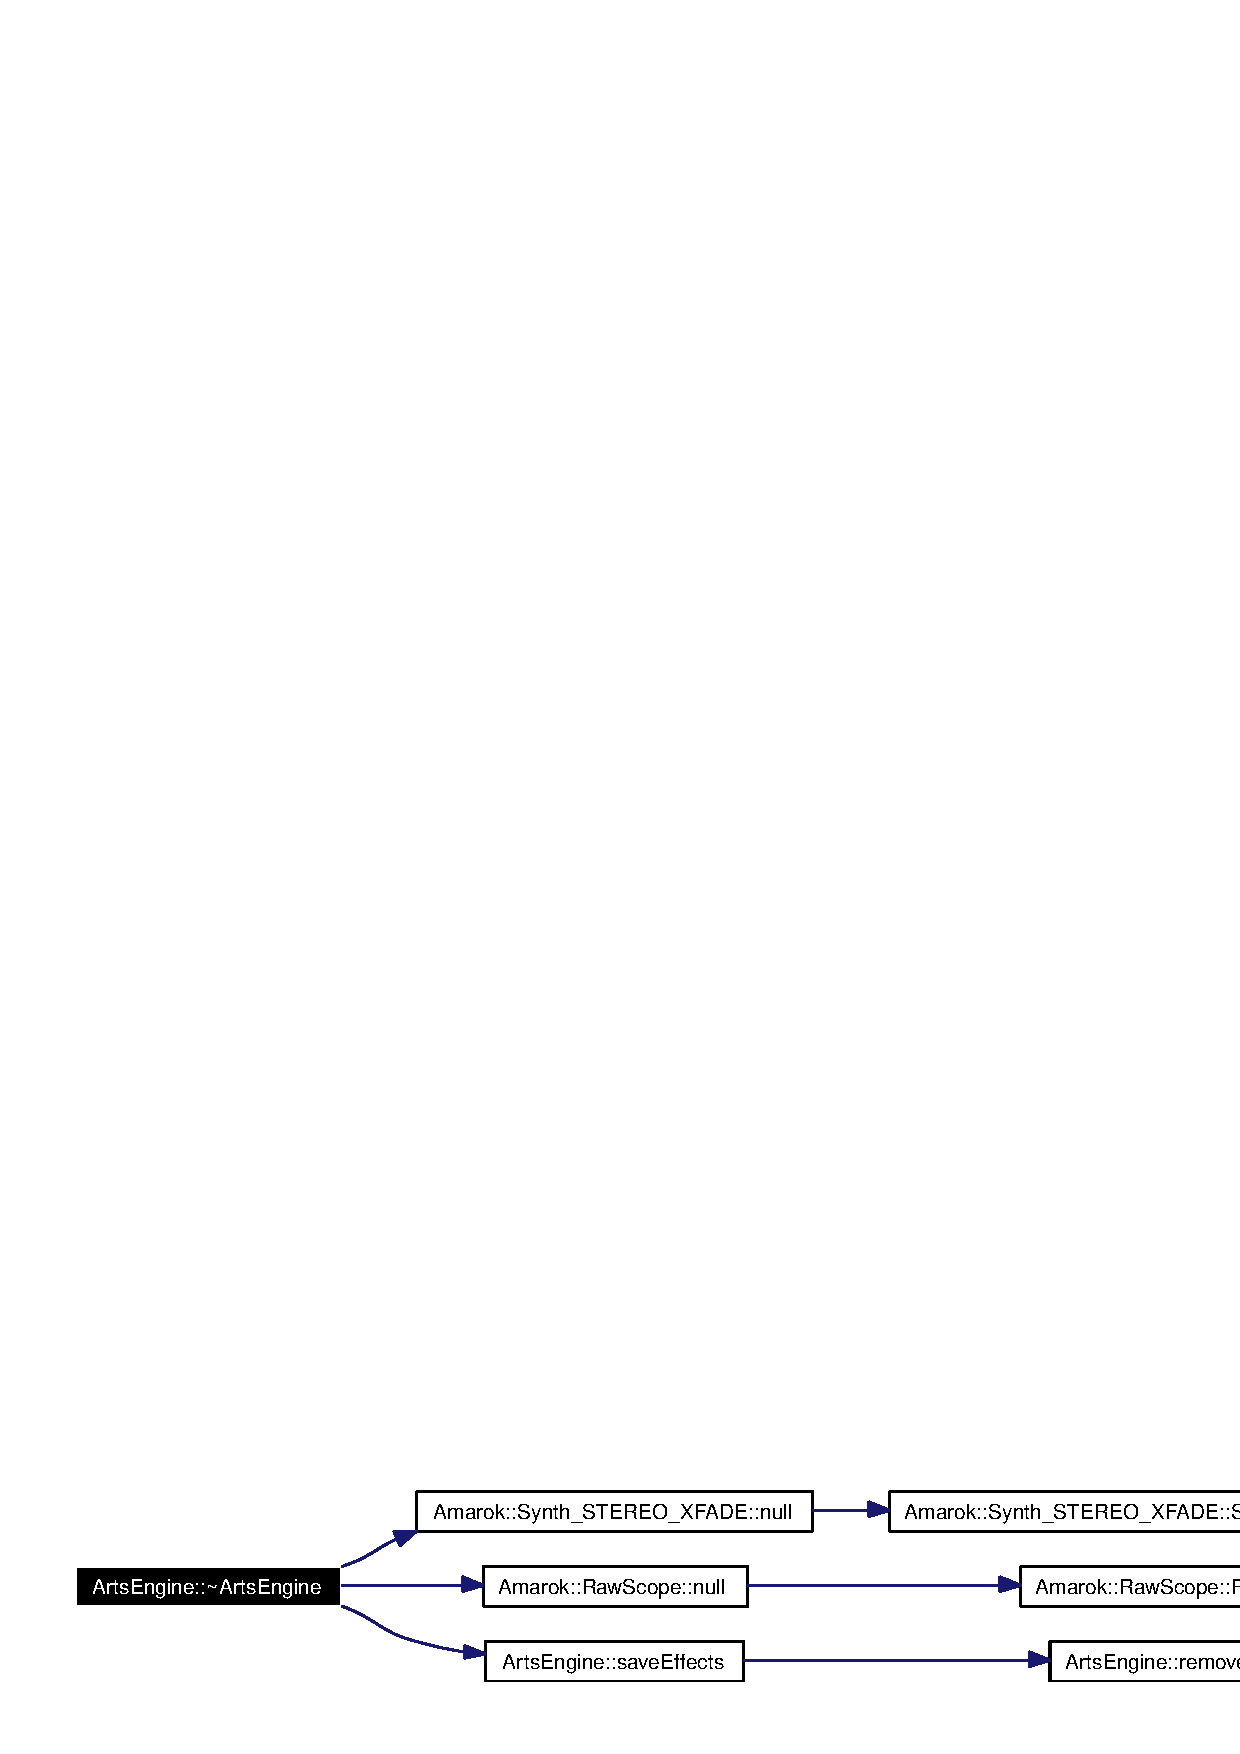
\includegraphics[width=356pt]{classArtsEngine_ArtsEnginea1_cgraph}
\end{center}
\end{figure}


\subsection{Member Function Documentation}
\index{ArtsEngine@{Arts\-Engine}!activeEffects@{activeEffects}}
\index{activeEffects@{activeEffects}!ArtsEngine@{Arts\-Engine}}
\subsubsection{\setlength{\rightskip}{0pt plus 5cm}std::vector$<$ long $>$ Arts\-Engine::active\-Effects () const\hspace{0.3cm}{\tt  [virtual]}}\label{classArtsEngine_ArtsEnginea11}




Reimplemented from {\bf Engine\-Base} {\rm (p.\,\pageref{classEngineBase_EngineBasea17})}.

Definition at line 498 of file artsengine.cpp.

References m\_\-effect\-Map.



\footnotesize\begin{verbatim}499 {
500     std::vector<long> vec;
501     QMap<long, EffectContainer>::ConstIterator it;
502 
503     for ( it = m_effectMap.begin(); it != m_effectMap.end(); ++it )
504     {
505         vec.push_back( it.key() );
506     }
507 
508     return vec;
509 }
\end{verbatim}\normalsize 
\index{ArtsEngine@{Arts\-Engine}!availableEffects@{availableEffects}}
\index{availableEffects@{availableEffects}!ArtsEngine@{Arts\-Engine}}
\subsubsection{\setlength{\rightskip}{0pt plus 5cm}QString\-List Arts\-Engine::available\-Effects () const\hspace{0.3cm}{\tt  [virtual]}}\label{classArtsEngine_ArtsEnginea10}




Reimplemented from {\bf Engine\-Base} {\rm (p.\,\pageref{classEngineBase_EngineBasea16})}.

Definition at line 478 of file artsengine.cpp.



\footnotesize\begin{verbatim}479 {
480     QStringList val;
481     Arts::TraderQuery query;
482     query.supports( "Interface", "Arts::StereoEffect" );
483     query.supports( "Interface", "Arts::SynthModule" );
484     std::vector<Arts::TraderOffer> *offers = query.query();
485 
486     for ( std::vector<Arts::TraderOffer>::iterator i = offers->begin(); i != offers->end(); i++ )
487     {
488         Arts::TraderOffer &offer = *i;
489         QCString name = offer.interfaceName().c_str();
490         val.append( name );
491     }
492     delete offers;
493 
494     return val;
495 }
\end{verbatim}\normalsize 
\index{ArtsEngine@{Arts\-Engine}!canDecode@{canDecode}}
\index{canDecode@{canDecode}!ArtsEngine@{Arts\-Engine}}
\subsubsection{\setlength{\rightskip}{0pt plus 5cm}bool Arts\-Engine::can\-Decode (const KURL \& {\em url}, mode\_\-t {\em mode}, mode\_\-t {\em permissions})\hspace{0.3cm}{\tt  [virtual]}}\label{classArtsEngine_ArtsEnginea4}




Implements {\bf Engine\-Base} {\rm (p.\,\pageref{classEngineBase_EngineBasea4})}.

Definition at line 284 of file artsengine.cpp.



\footnotesize\begin{verbatim}285 {
286     KFileItem fileItem( mode, permissions, url, false ); //false = determineMimeType straight away
287     KMimeType::Ptr mimetype = fileItem.determineMimeType();
288 
289     Arts::TraderQuery query;
290     query.supports( "Interface", "Arts::PlayObject" );
291     query.supports( "MimeType", mimetype->name().latin1() );
292     std::vector<Arts::TraderOffer> *offers = query.query();
293 
294     bool result = !offers->empty();
295     delete offers;
296 
297     return result;
298 }
\end{verbatim}\normalsize 
\index{ArtsEngine@{Arts\-Engine}!closeMixerHW@{closeMixerHW}}
\index{closeMixerHW@{closeMixerHW}!ArtsEngine@{Arts\-Engine}}
\subsubsection{\setlength{\rightskip}{0pt plus 5cm}void Engine\-Base::close\-Mixer\-HW ()\hspace{0.3cm}{\tt  [protected, inherited]}}\label{classEngineBase_EngineBaseb0}




Definition at line 61 of file enginebase.cpp.

References Engine\-Base::m\_\-mixer\-HW.

Referenced by init\-Mixer(), and Engine\-Base::$\sim$Engine\-Base().



\footnotesize\begin{verbatim}62 {
63     if ( m_mixerHW != -1 )
64     {
65         ::close( m_mixerHW );   //close /dev/mixer device
66         m_mixerHW = -1;
67     }
68 }
\end{verbatim}\normalsize 
\index{ArtsEngine@{Arts\-Engine}!configureDecoder@{configureDecoder}}
\index{configureDecoder@{configureDecoder}!ArtsEngine@{Arts\-Engine}}
\subsubsection{\setlength{\rightskip}{0pt plus 5cm}void Arts\-Engine::configure\-Decoder ()\hspace{0.3cm}{\tt  [virtual, slot]}}\label{classArtsEngine_ArtsEnginei6}




Reimplemented from {\bf Engine\-Base} {\rm (p.\,\pageref{classEngineBase_EngineBasei6})}.

Definition at line 614 of file artsengine.cpp.

References m\_\-p\-Decoder\-Config\-Widget, and m\_\-p\-Play\-Object.



\footnotesize\begin{verbatim}615 {
616     //this method shows a GUI for an aRts CODEC. currently only working with markey's modplug_artsplugin
617 
618     if ( m_pPlayObject && !m_pDecoderConfigWidget )
619     {
620         m_pDecoderConfigWidget = new ArtsConfigWidget( m_pPlayObject->object() );
621         connect( m_pPlayObject, SIGNAL( destroyed() ), m_pDecoderConfigWidget, SLOT( deleteLater() ) );
622 
623         m_pDecoderConfigWidget->show();
624     }
625 }
\end{verbatim}\normalsize 
\index{ArtsEngine@{Arts\-Engine}!configureEffect@{configureEffect}}
\index{configureEffect@{configureEffect}!ArtsEngine@{Arts\-Engine}}
\subsubsection{\setlength{\rightskip}{0pt plus 5cm}void Arts\-Engine::configure\-Effect (long {\em id})\hspace{0.3cm}{\tt  [virtual]}}\label{classArtsEngine_ArtsEnginea16}




Reimplemented from {\bf Engine\-Base} {\rm (p.\,\pageref{classEngineBase_EngineBasea22})}.

Definition at line 586 of file artsengine.cpp.

References m\_\-effect\-Map.



\footnotesize\begin{verbatim}587 {
588     if ( !m_effectMap[id].widget )
589     {
590         m_effectMap[id].widget = new ArtsConfigWidget( *m_effectMap[id].effect );
591         m_effectMap[id].widget->show();
592     }
593 }
\end{verbatim}\normalsize 
\index{ArtsEngine@{Arts\-Engine}!connectPlayObject@{connectPlayObject}}
\index{connectPlayObject@{connectPlayObject}!ArtsEngine@{Arts\-Engine}}
\subsubsection{\setlength{\rightskip}{0pt plus 5cm}void Arts\-Engine::connect\-Play\-Object ()\hspace{0.3cm}{\tt  [private, slot]}}\label{classArtsEngine_ArtsEnginek0}




Definition at line 385 of file artsengine.cpp.

References m\_\-p\-Connect\-Timer, m\_\-p\-Play\-Object, m\_\-xfade, m\_\-xfade\-Current, and m\_\-xfade\-Value.

Referenced by play().



\footnotesize\begin{verbatim}386 {
387     m_pConnectTimer->stop();
388 
389     if ( m_pPlayObject && !m_pPlayObject->isNull() && !m_pPlayObject->object().isNull() )
390     {
391         m_pPlayObject->object()._node()->start();
392 
393         //switch xfade channels
394         m_xfadeCurrent = ( m_xfadeCurrent == "invalue1" ) ? "invalue2" : "invalue1";
395 
396         if ( m_xfadeValue == 0.0 )
397             m_xfadeValue = 1.0;
398 
399         Arts::connect( m_pPlayObject->object(), "left", m_xfade, ( m_xfadeCurrent + "_l" ).latin1() );
400         Arts::connect( m_pPlayObject->object(), "right", m_xfade, ( m_xfadeCurrent + "_r" ).latin1() );
401     }
402 }
\end{verbatim}\normalsize 
\index{ArtsEngine@{Arts\-Engine}!connectTimeout@{connectTimeout}}
\index{connectTimeout@{connectTimeout}!ArtsEngine@{Arts\-Engine}}
\subsubsection{\setlength{\rightskip}{0pt plus 5cm}void Arts\-Engine::connect\-Timeout ()\hspace{0.3cm}{\tt  [private, slot]}}\label{classArtsEngine_ArtsEnginek1}




Definition at line 405 of file artsengine.cpp.

References m\_\-p\-Connect\-Timer, and m\_\-p\-Play\-Object.

Referenced by init(), and play().



\footnotesize\begin{verbatim}406 {
407     kdWarning() << "[ArtsEngine::connectTimeout()] Cannot initialize PlayObject! Skipping this track." << endl;
408     m_pConnectTimer->stop();
409 
410     delete m_pPlayObject;
411     m_pPlayObject = NULL;
412 }
\end{verbatim}\normalsize 
\index{ArtsEngine@{Arts\-Engine}!createEffect@{createEffect}}
\index{createEffect@{createEffect}!ArtsEngine@{Arts\-Engine}}
\subsubsection{\setlength{\rightskip}{0pt plus 5cm}long Arts\-Engine::create\-Effect (const QString \& {\em name})\hspace{0.3cm}{\tt  [virtual]}}\label{classArtsEngine_ArtsEnginea14}




Reimplemented from {\bf Engine\-Base} {\rm (p.\,\pageref{classEngineBase_EngineBasea20})}.

Definition at line 538 of file artsengine.cpp.

References Arts\-Engine::Effect\-Container::effect, m\_\-effect\-Map, m\_\-effect\-Stack, m\_\-server, and Arts\-Engine::Effect\-Container::widget.

Referenced by load\-Effects().



\footnotesize\begin{verbatim}539 {
540     const long error = 0;
541 
542     if ( name.isEmpty() )
543         return error;
544 
545     Arts::StereoEffect* pFX = new Arts::StereoEffect;
546     *pFX = Arts::DynamicCast( m_server.createObject( std::string( name.ascii() ) ) );
547 
548     if ( (*pFX).isNull() ) {
549         kdWarning() << "[ArtsEngine::createEffect] error: could not create effect." << endl;
550         delete pFX;
551         return error;
552     }
553 
554     pFX->start();
555     long id = m_effectStack.insertBottom( *pFX, std::string( name.ascii() ) );
556 
557     if ( !id ) {
558         kdWarning() << "[ArtsEngine::createEffect] error: insertBottom failed." << endl;
559         pFX->stop();
560         delete pFX;
561         return error;
562     }
563 
564     EffectContainer container;
565     container.effect = pFX;
566     container.widget = 0;
567 
568     m_effectMap.insert( id, container );
569 
570     return id;
571 }
\end{verbatim}\normalsize 
\index{ArtsEngine@{Arts\-Engine}!decoderConfigurable@{decoderConfigurable}}
\index{decoderConfigurable@{decoderConfigurable}!ArtsEngine@{Arts\-Engine}}
\subsubsection{\setlength{\rightskip}{0pt plus 5cm}virtual bool Engine\-Base::decoder\-Configurable () const\hspace{0.3cm}{\tt  [inline, virtual, inherited]}}\label{classEngineBase_EngineBasea23}




Definition at line 109 of file enginebase.h.



\footnotesize\begin{verbatim}109 { return false; }
\end{verbatim}\normalsize 
\index{ArtsEngine@{Arts\-Engine}!decoderConfigurable@{decoderConfigurable}}
\index{decoderConfigurable@{decoderConfigurable}!ArtsEngine@{Arts\-Engine}}
\subsubsection{\setlength{\rightskip}{0pt plus 5cm}bool Arts\-Engine::decoder\-Configurable ()}\label{classArtsEngine_ArtsEnginea17}




Definition at line 596 of file artsengine.cpp.

References m\_\-p\-Decoder\-Config\-Widget, and m\_\-p\-Play\-Object.



\footnotesize\begin{verbatim}597 {
598     if ( m_pPlayObject && !m_pPlayObject->object().isNull() && !m_pDecoderConfigWidget )
599     {
600         Arts::TraderQuery query;
601         query.supports( "Interface", "Arts::GuiFactory" );
602         query.supports( "CanCreate", m_pPlayObject->object()._interfaceName() );
603 
604         std::vector<Arts::TraderOffer> *queryResults = query.query();
605         bool yes = queryResults->size();
606         delete queryResults;
607 
608         return yes;
609     }
610     return false;
611 }
\end{verbatim}\normalsize 
\index{ArtsEngine@{Arts\-Engine}!effectConfigurable@{effectConfigurable}}
\index{effectConfigurable@{effectConfigurable}!ArtsEngine@{Arts\-Engine}}
\subsubsection{\setlength{\rightskip}{0pt plus 5cm}bool Arts\-Engine::effect\-Configurable (long {\em id}) const\hspace{0.3cm}{\tt  [virtual]}}\label{classArtsEngine_ArtsEnginea13}




Reimplemented from {\bf Engine\-Base} {\rm (p.\,\pageref{classEngineBase_EngineBasea19})}.

Definition at line 521 of file artsengine.cpp.

References m\_\-effect\-Map.



\footnotesize\begin{verbatim}522 {
523     if ( m_effectMap.find(id) == m_effectMap.end() )
524         return false;
525 
526     Arts::TraderQuery query;
527     query.supports( "Interface", "Arts::GuiFactory" );
528     query.supports( "CanCreate", (*m_effectMap[id].effect)._interfaceName() );
529 
530     std::vector<Arts::TraderOffer> *queryResults = query.query();
531     bool yes = queryResults->size();
532     delete queryResults;
533 
534     return yes;
535 }
\end{verbatim}\normalsize 
\index{ArtsEngine@{Arts\-Engine}!effectNameForId@{effectNameForId}}
\index{effectNameForId@{effectNameForId}!ArtsEngine@{Arts\-Engine}}
\subsubsection{\setlength{\rightskip}{0pt plus 5cm}QString Arts\-Engine::effect\-Name\-For\-Id (long {\em id}) const\hspace{0.3cm}{\tt  [virtual]}}\label{classArtsEngine_ArtsEnginea12}




Reimplemented from {\bf Engine\-Base} {\rm (p.\,\pageref{classEngineBase_EngineBasea18})}.

Definition at line 512 of file artsengine.cpp.

References m\_\-effect\-Map.



\footnotesize\begin{verbatim}513 {
514     const std::string str = (*m_effectMap[id].effect)._interfaceName();
515     QString qstr( str.c_str() );
516 
517     return qstr;
518 }
\end{verbatim}\normalsize 
\index{ArtsEngine@{Arts\-Engine}!endOfTrack@{endOfTrack}}
\index{endOfTrack@{endOfTrack}!ArtsEngine@{Arts\-Engine}}
\subsubsection{\setlength{\rightskip}{0pt plus 5cm}void Engine\-Base::end\-Of\-Track ()\hspace{0.3cm}{\tt  [signal, inherited]}}\label{classEngineBase_EngineBasel0}




Definition at line 113 of file enginebase.moc.



\footnotesize\begin{verbatim}114 {
115     activate_signal( staticMetaObject()->signalOffset() + 0 );
116 }
\end{verbatim}\normalsize 
\index{ArtsEngine@{Arts\-Engine}!getOutputsList@{getOutputsList}}
\index{getOutputsList@{getOutputsList}!ArtsEngine@{Arts\-Engine}}
\subsubsection{\setlength{\rightskip}{0pt plus 5cm}virtual QString\-List Engine\-Base::get\-Outputs\-List ()\hspace{0.3cm}{\tt  [inline, virtual, inherited]}}\label{classEngineBase_EngineBasea6}


Get list of available output plugins 

Definition at line 61 of file enginebase.h.



\footnotesize\begin{verbatim}61 { return QStringList(); }
\end{verbatim}\normalsize 
\index{ArtsEngine@{Arts\-Engine}!init@{init}}
\index{init@{init}!ArtsEngine@{Arts\-Engine}}
\subsubsection{\setlength{\rightskip}{0pt plus 5cm}void Arts\-Engine::init (bool \& {\em restart}, int {\em scope\-Size}, bool {\em restore\-Effects})\hspace{0.3cm}{\tt  [virtual]}}\label{classArtsEngine_ArtsEnginea2}




Implements {\bf Engine\-Base} {\rm (p.\,\pageref{classEngineBase_EngineBasea2})}.

Definition at line 104 of file artsengine.cpp.

References ARTS\_\-TIMER, Amarok::Raw\-Scope::buffer(), connect\-Timeout(), load\-Effects(), m\_\-aman\-Play, m\_\-effect\-Stack, m\_\-global\-Effect\-Stack, m\_\-p\-Connect\-Timer, m\_\-scope, m\_\-scope\-Id, m\_\-scope\-Size, m\_\-server, m\_\-xfade, m\_\-xfade\-Value, Amarok::Synth\_\-STEREO\_\-XFADE::percentage(), Amarok::Raw\-Scope::start(), and Amarok::Synth\_\-STEREO\_\-XFADE::start().



\footnotesize\begin{verbatim}105 {
106     kdDebug() << "BEGIN " << k_funcinfo << endl;
107 
108     m_scopeSize = 1 << scopeSize;   
109     m_restoreEffects = restoreEffects;
110     m_mixerHW = -1;   //initialize
111 
112     // We must restart artsd whenever we installed new mcopclasses
113     if ( restart )
114     {
115         QCString kill_cmdline;
116         kill_cmdline = "killall artsd";
117 
118         int kill_status = ::system( kill_cmdline );
119         if ( kill_status != -1 && WIFEXITED( kill_status ) )
120         {
121             kdWarning() << "killall artsd succeeded." << endl;
122             restart = false;
123         }
124     }
125 
126     KConfig config( "kcmartsrc" );
127     config.setGroup( "Arts" );
128 
129     bool realtime = config.readBoolEntry( "StartRealtime", true );
130 
131     if ( !realtime )
132         KMessageBox::information( 0, i18n( "<p>artsd is not running with <b>realtime priority</b> which may cause audio playback to \"skip\" and stutter.<p>"
133                                      "<p>To use realtime priority, open the KDE Control Center and enable \"Run with highest possible priority\", under <i>Sound System</i> in the <i>Sound & Multimedia</i> branch. "
134                                      "Some people may also have to check that \"$KDEDIR/bin/artswrapper\" is <b>set suid</b> (chmod +s).</p>"
135                                      "<p>You may find, however, that playback is fine without increasing the priority of artsd.</p>" ),
136                                i18n( "aRts Problem" ), "artsRealtimeAdvice" );
137 
138     m_server = Arts::Reference( "global:Arts_SoundServerV2" );
139 
140     if ( m_server.isNull() || m_server.error() )
141     {
142         kdWarning() << "aRtsd not running.. trying to start" << endl;
143         // aRts seems not to be running, let's try to run it
144         // First, let's read the configuration as in kcmarts
145         QCString cmdline;
146 
147         bool x11Comm = config.readBoolEntry( "X11GlobalComm", false );
148 
149         // put the value of x11Comm into .mcoprc
150         {
151             KConfig X11CommConfig( QDir::homeDirPath() + "/.mcoprc" );
152 
153             if ( x11Comm )
154                 X11CommConfig.writeEntry( "GlobalComm", "Arts::X11GlobalComm" );
155             else
156                 X11CommConfig.writeEntry( "GlobalComm", "Arts::TmpGlobalComm" );
157 
158             X11CommConfig.sync();
159         }
160 
161         cmdline = QFile::encodeName( KStandardDirs::findExe( QString::fromLatin1( "kdeinit_wrapper" ) ) );
162         cmdline += " ";
163 
164         if ( realtime )
165             cmdline += QFile::encodeName( KStandardDirs::findExe(
166                                               QString::fromLatin1( "artswrapper" ) ) );
167         else
168             cmdline += QFile::encodeName( KStandardDirs::findExe(
169                                               QString::fromLatin1( "artsd" ) ) );
170 
171         cmdline += " ";
172         cmdline += config.readEntry( "Arguments", "-F 10 -S 4096 -s 60 -m artsmessage -l 3 -f -n" ).utf8();
173 
174         int status = ::system( cmdline );
175 
176         if ( status != -1 && WIFEXITED( status ) )
177         {
178             // We could have a race-condition here.
179             // The correct way to do it is to make artsd fork-and-exit
180             // after starting to listen to connections (and running artsd
181             // directly instead of using kdeinit), but this is better
182             // than nothing.
183             int time = 0;
184             do
185             {
186                 // every time it fails, we should wait a little longer
187                 // between tries
188                 ::sleep( 1 + time / 2 );
189                 m_server = Arts::Reference( "global:Arts_SoundServerV2" );
190             }
191             while ( ++time < 5 && ( m_server.isNull() ) );
192         }
193     }
194 
195     if ( m_server.isNull() )
196     {
197         KMessageBox::error( 0, i18n( "Cannot start aRts. Exiting." ), i18n( "Fatal Error" ) );
198         ::exit( 1 );
199     }
200 
201     { //amanPlay
202         m_amanPlay = Arts::DynamicCast( m_server.createObject( "Arts::Synth_AMAN_PLAY" ) );
203         m_amanPlay.title( "amarok" );
204         m_amanPlay.autoRestoreID( "amarok" );
205         m_amanPlay.start();
206     }
207 
208     { //Xfade
209         m_xfade = Arts::DynamicCast( m_server.createObject( "Amarok::Synth_STEREO_XFADE" ) );
210 
211         if ( m_xfade.isNull() ) {
212             KMessageBox::error( 0,
213                                 i18n( "<p>There was an error loading libamarokarts. First try:"
214                                       "<pre>killall -9 artsd && amarok</pre>"
215                                       "If that does not work then amaroK was probably installed with the wrong prefix; "
216                                       "please re-configure amaroK using:"
217                                       "<pre>./configure --prefix=`kde-config --prefix` && su -c \"make install\"</pre>" ),
218                                 i18n( "Fatal Error" ) );
219             ::exit( 1 );
220         }
221 
222         m_xfade.percentage( m_xfadeValue );
223         m_xfade.start();
224     }
225 
226     { //globalEffectStack
227         m_globalEffectStack = Arts::DynamicCast( m_server.createObject( "Arts::StereoEffectStack" ) );
228         m_globalEffectStack.start();
229     }
230 
231     { //effectStack
232         m_effectStack = Arts::DynamicCast( m_server.createObject( "Arts::StereoEffectStack" ) );
233         m_effectStack.start();
234         m_globalEffectStack.insertBottom( m_effectStack, "Effect Stack" );
235     }
236 
237     { //scope
238         m_scope = Arts::DynamicCast( m_server.createObject( "Amarok::RawScope" ) );
239         m_scope.start();
240         m_scope.buffer( m_scopeSize );
241         m_scopeId = m_globalEffectStack.insertTop( m_scope, "Analyzer" );
242     }
243 
244     Arts::connect( m_globalEffectStack  , m_amanPlay );
245     Arts::connect( m_xfade, "outvalue_l", m_globalEffectStack, "inleft" );
246     Arts::connect( m_xfade, "outvalue_r", m_globalEffectStack, "inright" );
247 
248     if ( m_restoreEffects ) loadEffects();
249     startTimer( ARTS_TIMER );
250     connect( m_pConnectTimer, SIGNAL( timeout() ), this, SLOT( connectTimeout() ) );
251 
252     kdDebug() << "END " << k_funcinfo << endl;
253     
254 }
\end{verbatim}\normalsize 


Here is the call graph for this function:\begin{figure}[H]
\begin{center}
\leavevmode
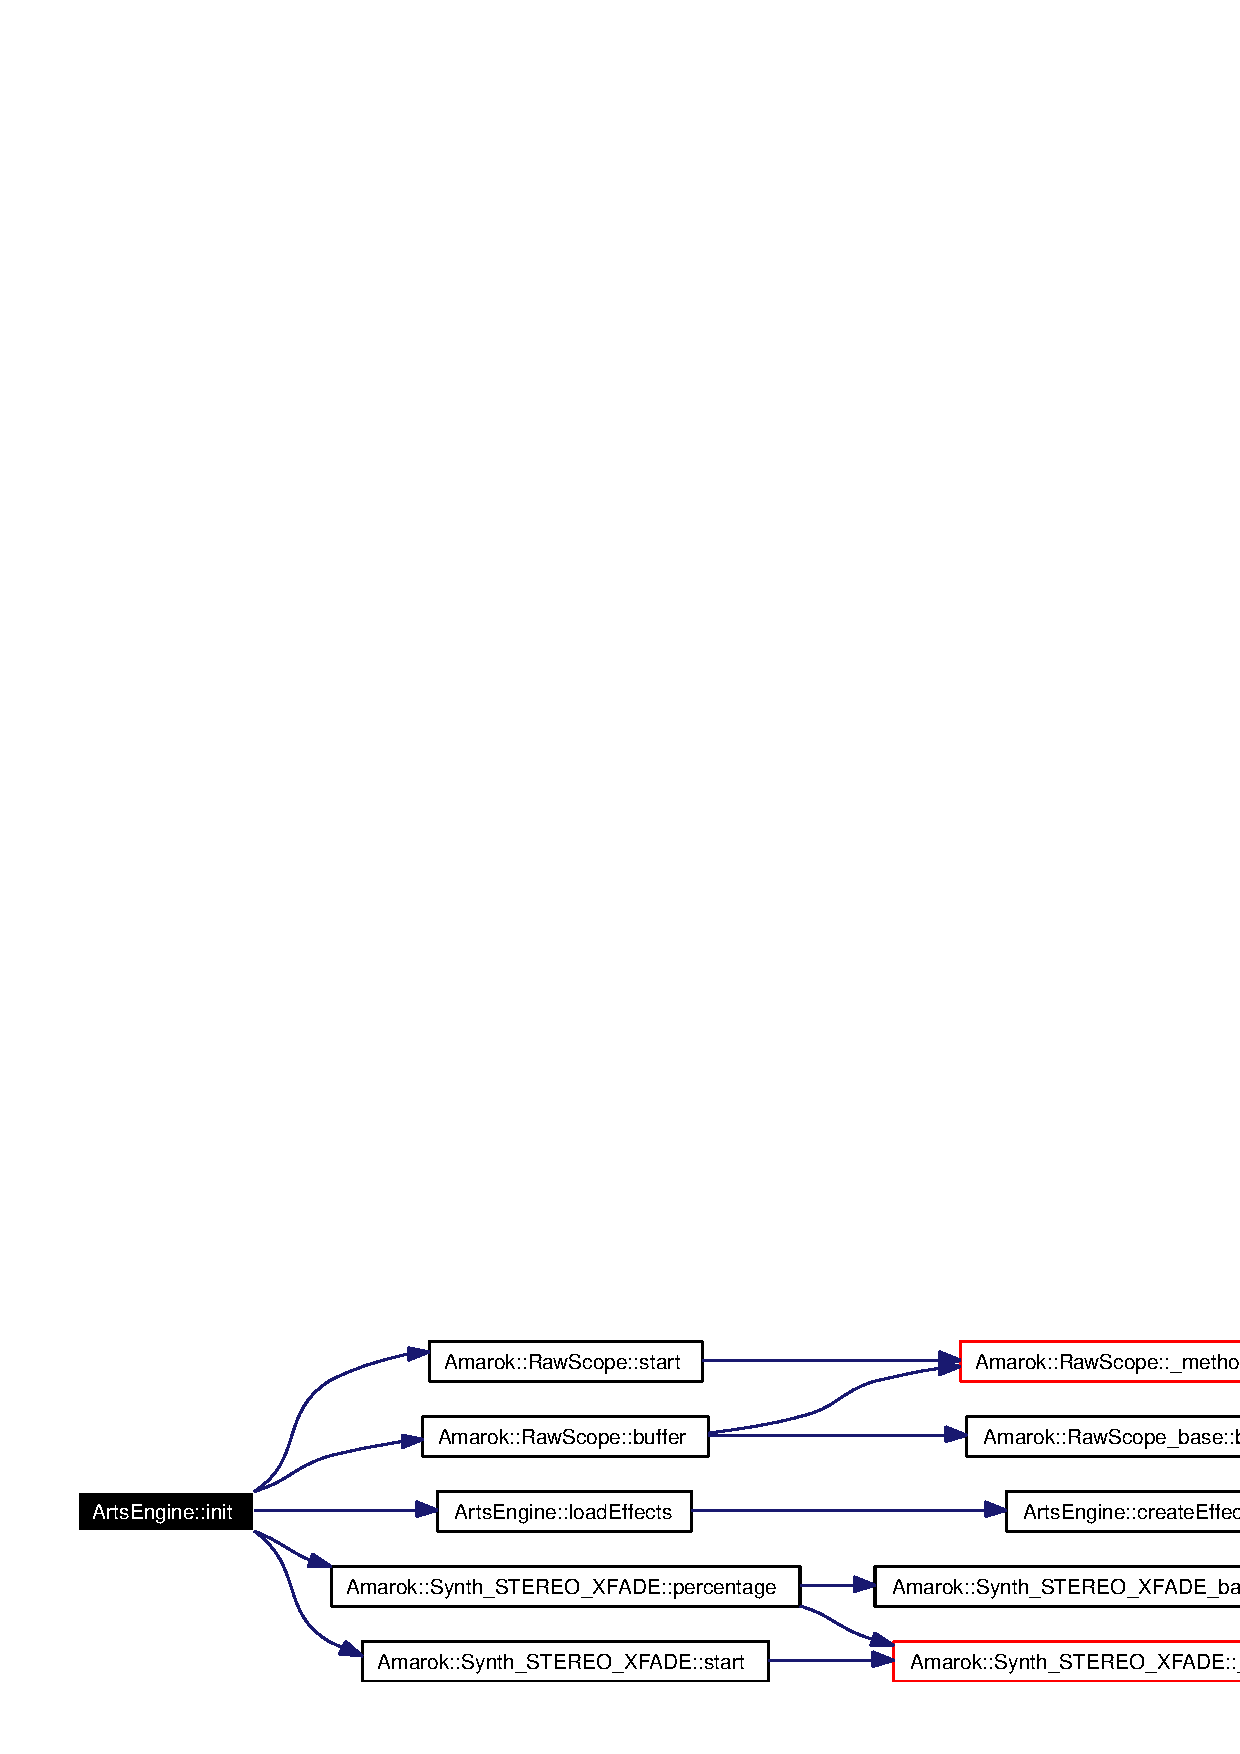
\includegraphics[width=336pt]{classArtsEngine_ArtsEnginea2_cgraph}
\end{center}
\end{figure}
\index{ArtsEngine@{Arts\-Engine}!initMixer@{initMixer}}
\index{initMixer@{initMixer}!ArtsEngine@{Arts\-Engine}}
\subsubsection{\setlength{\rightskip}{0pt plus 5cm}bool Arts\-Engine::init\-Mixer (bool {\em hardware})\hspace{0.3cm}{\tt  [virtual]}}\label{classArtsEngine_ArtsEnginea3}


Initialize mixer. \begin{Desc}
\item[Parameters:]
\begin{description}
\item[{\em hardware}]True for soundcard hardware mixing \end{description}
\end{Desc}
\begin{Desc}
\item[Returns:]True if using hardware mixing \end{Desc}


Implements {\bf Engine\-Base} {\rm (p.\,\pageref{classEngineBase_EngineBasea3})}.

Definition at line 257 of file artsengine.cpp.

References Engine\-Base::close\-Mixer\-HW(), Engine\-Base::init\-Mixer\-HW(), m\_\-global\-Effect\-Stack, m\_\-server, m\_\-volume\-Control, and m\_\-volume\-Id.



\footnotesize\begin{verbatim}258 {
259     { //make sure any previously started volume control gets killed
260         if ( m_volumeId )
261         {
262             m_globalEffectStack.remove( m_volumeId );
263             m_volumeId = 0;
264             m_volumeControl = Arts::StereoVolumeControl::null();
265         }
266         closeMixerHW();
267     }
268 
269     if ( hardware )
270         hardware = initMixerHW();
271     else
272     {
273         m_volumeControl = Arts::DynamicCast( m_server.createObject( "Arts::StereoVolumeControl" ) );
274         m_volumeControl.start();
275         m_volumeId = m_globalEffectStack.insertBottom( m_volumeControl, "Volume Control" );
276     }
277     return hardware;
278 }
\end{verbatim}\normalsize 


Here is the call graph for this function:\begin{figure}[H]
\begin{center}
\leavevmode
\includegraphics[width=161pt]{classArtsEngine_ArtsEnginea3_cgraph}
\end{center}
\end{figure}
\index{ArtsEngine@{Arts\-Engine}!initMixerHW@{initMixerHW}}
\index{initMixerHW@{initMixerHW}!ArtsEngine@{Arts\-Engine}}
\subsubsection{\setlength{\rightskip}{0pt plus 5cm}bool Engine\-Base::init\-Mixer\-HW ()\hspace{0.3cm}{\tt  [protected, inherited]}}\label{classEngineBase_EngineBaseb1}




Definition at line 43 of file enginebase.cpp.

References Engine\-Base::m\_\-mixer\-HW.

Referenced by init\-Mixer().



\footnotesize\begin{verbatim}44 {
45     if ( ( m_mixerHW = ::open( "/dev/mixer", O_RDWR ) ) < 0 )
46         return false;  //failed
47     else
48     {
49         int devmask, recmask, i_recsrc, stereodevs;
50         if ( ioctl( m_mixerHW, SOUND_MIXER_READ_DEVMASK, &devmask )       == -1 ) return false;
51         if ( ioctl( m_mixerHW, SOUND_MIXER_READ_RECMASK, &recmask )       == -1 ) return false;
52         if ( ioctl( m_mixerHW, SOUND_MIXER_READ_RECSRC, &i_recsrc )       == -1 ) return false;
53         if ( ioctl( m_mixerHW, SOUND_MIXER_READ_STEREODEVS, &stereodevs ) == -1 ) return false;
54         if ( !devmask )                                                           return false;
55     }
56 
57     return true;
58 }
\end{verbatim}\normalsize 
\index{ArtsEngine@{Arts\-Engine}!isMixerHardware@{isMixerHardware}}
\index{isMixerHardware@{isMixerHardware}!ArtsEngine@{Arts\-Engine}}
\subsubsection{\setlength{\rightskip}{0pt plus 5cm}bool Engine\-Base::is\-Mixer\-Hardware () const\hspace{0.3cm}{\tt  [inline, inherited]}}\label{classEngineBase_EngineBasea11}


Sets the master volume. \begin{Desc}
\item[Returns:]True if using hardware mixer. \end{Desc}


Definition at line 85 of file enginebase.h.

References Engine\-Base::m\_\-mixer\-HW.



\footnotesize\begin{verbatim}85 { return m_mixerHW != -1; }
\end{verbatim}\normalsize 
\index{ArtsEngine@{Arts\-Engine}!isStream@{isStream}}
\index{isStream@{isStream}!ArtsEngine@{Arts\-Engine}}
\subsubsection{\setlength{\rightskip}{0pt plus 5cm}bool Arts\-Engine::is\-Stream () const\hspace{0.3cm}{\tt  [virtual]}}\label{classArtsEngine_ArtsEnginea8}




Implements {\bf Engine\-Base} {\rm (p.\,\pageref{classEngineBase_EngineBasea12})}.

Definition at line 333 of file artsengine.cpp.

References m\_\-p\-Play\-Object.



\footnotesize\begin{verbatim}334 {
335     if ( m_pPlayObject )
336         return m_pPlayObject->stream();
337     else
338         return false;
339 }
\end{verbatim}\normalsize 
\index{ArtsEngine@{Arts\-Engine}!loaded@{loaded}}
\index{loaded@{loaded}!ArtsEngine@{Arts\-Engine}}
\subsubsection{\setlength{\rightskip}{0pt plus 5cm}bool Engine\-Base::loaded ()\hspace{0.3cm}{\tt  [inline, inherited]}}\label{classEngineBase_EngineBasea9}


\begin{Desc}
\item[Returns:]True if media is loaded, system is ready to play. \end{Desc}


Definition at line 73 of file enginebase.h.

References Engine\-Base::Empty, and Engine\-Base::state().

Referenced by Engine\-Controller::pause().



\footnotesize\begin{verbatim}73 { return state() != Empty; }
\end{verbatim}\normalsize 


Here is the call graph for this function:\begin{figure}[H]
\begin{center}
\leavevmode
\includegraphics[width=138pt]{classEngineBase_EngineBasea9_cgraph}
\end{center}
\end{figure}
\index{ArtsEngine@{Arts\-Engine}!loadEffects@{loadEffects}}
\index{loadEffects@{loadEffects}!ArtsEngine@{Arts\-Engine}}
\subsubsection{\setlength{\rightskip}{0pt plus 5cm}void Arts\-Engine::load\-Effects ()\hspace{0.3cm}{\tt  [private]}}\label{classArtsEngine_ArtsEngined2}




Definition at line 672 of file artsengine.cpp.

References create\-Effect(), and m\_\-effect\-Map.

Referenced by init().



\footnotesize\begin{verbatim}673 {
674     kdDebug() << k_funcinfo << endl;
675 
676     QDomDocument doc;
677     assert( kapp );
678     QFile file( kapp->dirs()->saveLocation( "data", kapp->instanceName() + "/" ) + "arts-effects.xml" );
679 
680     if ( !file.open( IO_ReadOnly ) )
681     {
682         kdWarning() << "[ArtsEngine::loadEffects()] error: !file.open()" << endl;
683         return;
684     }
685 
686     QString errorMsg;
687     int     errorLine;
688     int     errorColumn;
689     if ( !doc.setContent( &file, &errorMsg, &errorLine, &errorColumn ) )
690     {
691         kdWarning() << "[ArtsEngine::loadEffects()] error: !doc.setContent()" << endl;
692         kdWarning() << "[ArtsEngine::loadEffects()] errorMsg   : " << errorMsg    << endl;
693         kdWarning() << "[ArtsEngine::loadEffects()] errorLine  : " << errorLine   << endl;
694         kdWarning() << "[ArtsEngine::loadEffects()] errorColumn: " << errorColumn << endl;
695         file.close();
696         return;
697     }
698 
699     QDomElement docElem = doc.documentElement();
700 
701     for ( QDomNode n = docElem.firstChild(); !n.isNull(); n = n.nextSibling() )
702     {
703         QString effect = n.namedItem( "effectname" ).firstChild().toText().nodeValue();
704         kdDebug() << "effectname: " << effect << endl;
705 
706         long id = createEffect( effect );
707         for ( QDomNode nAttr = n.firstChild(); id && !nAttr.isNull(); nAttr = nAttr.nextSibling() )
708         {
709             if ( nAttr.nodeName() == "attribute" )
710             {
711                 QString name  = nAttr.namedItem( "name"  ).firstChild().toText().nodeValue();
712                 QString type  = nAttr.namedItem( "type"  ).firstChild().toText().nodeValue();
713                 QString value = nAttr.namedItem( "value" ).firstChild().toText().nodeValue();
714 
715                 kdDebug() << "name : " << name  << endl;
716                 kdDebug() << "type : " << type  << endl;
717                 kdDebug() << "value: " << value << endl;
718 
719                 Arts::DynamicRequest req( *m_effectMap[id].effect );
720                 std::string set( "_set_" );
721                 set.append( std::string( name.latin1() ) );
722                 req.method( set );
723 
724                 Arts::Buffer buf;
725                 buf.fromString( std::string( value.latin1() ), "" );
726 
727                 Arts::Any param;
728                 param.type = std::string( type.latin1() );
729                 param.readType( buf );
730                 req.param( param );
731 
732                 if ( !req.invoke() )
733                     kdWarning() << "DynamicRequest failed." << endl;
734             }
735         }
736     }
737 }
\end{verbatim}\normalsize 


Here is the call graph for this function:\begin{figure}[H]
\begin{center}
\leavevmode
\includegraphics[width=160pt]{classArtsEngine_ArtsEngined2_cgraph}
\end{center}
\end{figure}
\index{ArtsEngine@{Arts\-Engine}!newStreamData@{newStreamData}}
\index{newStreamData@{newStreamData}!ArtsEngine@{Arts\-Engine}}
\subsubsection{\setlength{\rightskip}{0pt plus 5cm}virtual void Engine\-Base::new\-Stream\-Data (char $\ast$, int)\hspace{0.3cm}{\tt  [inline, virtual, slot, inherited]}}\label{classEngineBase_EngineBasei7}




Definition at line 130 of file enginebase.h.



\footnotesize\begin{verbatim}130 {};
\end{verbatim}\normalsize 
\index{ArtsEngine@{Arts\-Engine}!pause@{pause}}
\index{pause@{pause}!ArtsEngine@{Arts\-Engine}}
\subsubsection{\setlength{\rightskip}{0pt plus 5cm}void Arts\-Engine::pause ()\hspace{0.3cm}{\tt  [virtual, slot]}}\label{classArtsEngine_ArtsEnginei3}




Implements {\bf Engine\-Base} {\rm (p.\,\pageref{classEngineBase_EngineBasei3})}.

Definition at line 440 of file artsengine.cpp.

References m\_\-p\-Play\-Object.



\footnotesize\begin{verbatim}441 {
442     if ( m_pPlayObject )
443     {
444         m_pPlayObject->pause();
445     }
446 }
\end{verbatim}\normalsize 
\index{ArtsEngine@{Arts\-Engine}!play@{play}}
\index{play@{play}!ArtsEngine@{Arts\-Engine}}
\subsubsection{\setlength{\rightskip}{0pt plus 5cm}void Arts\-Engine::play ()\hspace{0.3cm}{\tt  [virtual, slot]}}\label{classArtsEngine_ArtsEnginei1}




Implements {\bf Engine\-Base} {\rm (p.\,\pageref{classEngineBase_EngineBasei1})}.

Definition at line 415 of file artsengine.cpp.

References m\_\-p\-Play\-Object.

Referenced by play().



\footnotesize\begin{verbatim}416 {
417     if ( m_pPlayObject )
418     {   
419         qWarning("Arts Play files");  
420         m_pPlayObject->play();
421     }
422 }
\end{verbatim}\normalsize 
\index{ArtsEngine@{Arts\-Engine}!play@{play}}
\index{play@{play}!ArtsEngine@{Arts\-Engine}}
\subsubsection{\setlength{\rightskip}{0pt plus 5cm}void Arts\-Engine::play (const KURL \&)\hspace{0.3cm}{\tt  [virtual, slot]}}\label{classArtsEngine_ArtsEnginei0}




Implements {\bf Engine\-Base} {\rm (p.\,\pageref{classEngineBase_EngineBasei0})}.

Definition at line 349 of file artsengine.cpp.

References connect\-Play\-Object(), connect\-Timeout(), m\_\-p\-Connect\-Timer, m\_\-p\-Play\-Object, m\_\-server, m\_\-xfade\-Fadeout, play(), start\-Xfade(), Engine\-Base::stopped(), and TIMEOUT.



\footnotesize\begin{verbatim}350 {
351     kdDebug() << k_funcinfo << endl;
352     m_xfadeFadeout = false;
353     startXfade();
354     KDE::PlayObjectFactory factory( m_server );
355     m_pPlayObject = factory.createPlayObject( url, false ); //second parameter: create BUS(true/false)
356 
357     if ( !m_pPlayObject || m_pPlayObject->isNull() ) 
358     {
359         qWarning("Arts Error 1----------------");
360         connectTimeout();
361         emit stopped();
362     }
363     else
364     {      
365         connect( m_pPlayObject, SIGNAL( destroyed() ), this, SIGNAL( stopped() ) );
366 
367         if ( m_pPlayObject->object().isNull() ) 
368         {
369             kdDebug() << k_funcinfo << " m_pPlayObject->object().isNull()" << endl;
370             qWarning("Arts Error 2----------------");
371             connect( m_pPlayObject, SIGNAL( playObjectCreated() ), this, SLOT( connectPlayObject() ) );
372             m_pConnectTimer->start( TIMEOUT, true );
373         }
374         else 
375         {
376             connectPlayObject();
377              qWarning("Arts Connect");
378         }
379 
380         play();
381     }
382 }
\end{verbatim}\normalsize 
\index{ArtsEngine@{Arts\-Engine}!position@{position}}
\index{position@{position}!ArtsEngine@{Arts\-Engine}}
\subsubsection{\setlength{\rightskip}{0pt plus 5cm}long Arts\-Engine::position () const\hspace{0.3cm}{\tt  [virtual]}}\label{classArtsEngine_ArtsEnginea6}


\begin{Desc}
\item[Returns:]Time position in ms \end{Desc}


Implements {\bf Engine\-Base} {\rm (p.\,\pageref{classEngineBase_EngineBasea7})}.

Definition at line 301 of file artsengine.cpp.

References m\_\-p\-Play\-Object.



\footnotesize\begin{verbatim}302 {
303     if ( m_pPlayObject )
304         return m_pPlayObject->currentTime().seconds * 1000 +
305                m_pPlayObject->currentTime().ms;
306     else
307         return 0;
308 }
\end{verbatim}\normalsize 
\index{ArtsEngine@{Arts\-Engine}!removeEffect@{removeEffect}}
\index{removeEffect@{removeEffect}!ArtsEngine@{Arts\-Engine}}
\subsubsection{\setlength{\rightskip}{0pt plus 5cm}void Arts\-Engine::remove\-Effect (long {\em id})\hspace{0.3cm}{\tt  [virtual]}}\label{classArtsEngine_ArtsEnginea15}




Reimplemented from {\bf Engine\-Base} {\rm (p.\,\pageref{classEngineBase_EngineBasea21})}.

Definition at line 574 of file artsengine.cpp.

References m\_\-effect\-Map, and m\_\-effect\-Stack.

Referenced by save\-Effects().



\footnotesize\begin{verbatim}575 {
576     m_effectStack.remove( id );
577 
578     m_effectMap[id].effect->stop();
579     delete m_effectMap[id].widget;
580     delete m_effectMap[id].effect;
581 
582     m_effectMap.remove( id );
583 }
\end{verbatim}\normalsize 
\index{ArtsEngine@{Arts\-Engine}!saveEffects@{saveEffects}}
\index{saveEffects@{saveEffects}!ArtsEngine@{Arts\-Engine}}
\subsubsection{\setlength{\rightskip}{0pt plus 5cm}void Arts\-Engine::save\-Effects ()\hspace{0.3cm}{\tt  [private]}}\label{classArtsEngine_ArtsEngined3}




Definition at line 740 of file artsengine.cpp.

References m\_\-effect\-Map, and remove\-Effect().

Referenced by $\sim$Arts\-Engine().



\footnotesize\begin{verbatim}741 {
742     QDomDocument doc;
743     QDomElement root = doc.createElement( "aRts-Effects" );
744     doc.appendChild( root );
745 
746     for ( QMap<long, EffectContainer>::Iterator it = m_effectMap.begin(); it != m_effectMap.end(); ++it )
747     {
748         QDomElement tagEffect = doc.createElement( "effect" );
749         root.appendChild( tagEffect );
750 
751             { //effectname
752                 QDomElement tag = doc.createElement( "effectname" );
753                 tagEffect.appendChild( tag );
754                 QDomText txt = doc.createTextNode( (*it.data().effect)._interfaceName().c_str() );
755                 tag.appendChild( txt );
756             }
757 
758         Arts::InterfaceDef def = (*it.data().effect)._queryInterface( (*it.data().effect)._interfaceName() );
759 
760         for ( uint i = 0; i < def.attributes.size(); i++ )
761         {
762             QDomElement tagAttribute = doc.createElement( "attribute" );
763             tagEffect.appendChild( tagAttribute );
764 
765             { //name
766                 QDomElement tag = doc.createElement( "name" );
767                 tagAttribute.appendChild( tag );
768                 QDomText txt = doc.createTextNode( def.attributes[i].name.c_str() );
769                 tag.appendChild( txt );
770             }
771 
772             Arts::DynamicRequest req( *it.data().effect );
773             req.method( "_get_" + def.attributes[i].name );
774             Arts::Any result;
775             result.type = def.attributes[i].type;
776 
777             { //type
778                 QDomElement tag = doc.createElement( "type" );
779                 tagAttribute.appendChild( tag );
780                 QDomText txt = doc.createTextNode( def.attributes[i].type.c_str() );
781                 tag.appendChild( txt );
782             }
783 
784             if ( !req.invoke( result ) )
785                 kdWarning() << "request failed." << endl;
786 
787             Arts::Buffer buf;
788             result.writeType( buf );
789 
790             { //value
791                 QDomElement tag = doc.createElement( "value" );
792                 tagAttribute.appendChild( tag );
793                 QDomText txt = doc.createTextNode( buf.toString( "" ).c_str() );
794                 tag.appendChild( txt );
795             }
796         }
797         removeEffect( it.key() );
798     }
799 
800     assert( kapp );
801     QString path = kapp->dirs()->saveLocation( "data", kapp->instanceName() + "/" ) + "arts-effects.xml";
802     QFile::remove( path );
803     QFile file( path );
804     file.open( IO_ReadWrite );
805     QTextStream stream( &file );
806     stream << doc;
807 }
\end{verbatim}\normalsize 


Here is the call graph for this function:\begin{figure}[H]
\begin{center}
\leavevmode
\includegraphics[width=164pt]{classArtsEngine_ArtsEngined3_cgraph}
\end{center}
\end{figure}
\index{ArtsEngine@{Arts\-Engine}!scope@{scope}}
\index{scope@{scope}!ArtsEngine@{Arts\-Engine}}
\subsubsection{\setlength{\rightskip}{0pt plus 5cm}std::vector$<$ float $>$ $\ast$ Arts\-Engine::scope ()\hspace{0.3cm}{\tt  [virtual]}}\label{classArtsEngine_ArtsEnginea9}


Fetches the current audio sample buffer. \begin{Desc}
\item[Returns:]Pointer to result of FFT calculation. Must be deleted after use. \end{Desc}


Reimplemented from {\bf Engine\-Base} {\rm (p.\,\pageref{classEngineBase_EngineBasea14})}.

Definition at line 342 of file artsengine.cpp.

References m\_\-scope, and Amarok::Raw\-Scope::scope().



\footnotesize\begin{verbatim}343 {
344     return m_scope.scope();
345 }
\end{verbatim}\normalsize 


Here is the call graph for this function:\begin{figure}[H]
\begin{center}
\leavevmode
\includegraphics[width=359pt]{classArtsEngine_ArtsEnginea9_cgraph}
\end{center}
\end{figure}
\index{ArtsEngine@{Arts\-Engine}!seek@{seek}}
\index{seek@{seek}!ArtsEngine@{Arts\-Engine}}
\subsubsection{\setlength{\rightskip}{0pt plus 5cm}void Arts\-Engine::seek (long {\em ms})\hspace{0.3cm}{\tt  [virtual, slot]}}\label{classArtsEngine_ArtsEnginei4}




Implements {\bf Engine\-Base} {\rm (p.\,\pageref{classEngineBase_EngineBasei5})}.

Definition at line 449 of file artsengine.cpp.

References m\_\-p\-Play\-Object.



\footnotesize\begin{verbatim}450 {
451 kdDebug() << "seek" << ms << endl;
452     if ( m_pPlayObject )
453     {
454     kdDebug() << "if ~~~seek" << ms << endl;
455         Arts::poTime time;
456         time.ms      = ms % 1000;
457         time.seconds = ( ms - time.ms ) / 1000;
458         time.custom  = 0.0;
459         m_pPlayObject->seek( time );
460     }
461 }
\end{verbatim}\normalsize 
\index{ArtsEngine@{Arts\-Engine}!setDefaultSoundDevice@{setDefaultSoundDevice}}
\index{setDefaultSoundDevice@{setDefaultSoundDevice}!ArtsEngine@{Arts\-Engine}}
\subsubsection{\setlength{\rightskip}{0pt plus 5cm}virtual void Engine\-Base::set\-Default\-Sound\-Device (bool {\em is\-Default})\hspace{0.3cm}{\tt  [inline, virtual, inherited]}}\label{classEngineBase_EngineBasea27}




Definition at line 114 of file enginebase.h.

References Engine\-Base::m\_\-default\-Sound\-Device.

Referenced by Myplayer::Myplayer().



\footnotesize\begin{verbatim}114 { m_defaultSoundDevice = isDefault; }
\end{verbatim}\normalsize 
\index{ArtsEngine@{Arts\-Engine}!setRestoreEffects@{setRestoreEffects}}
\index{setRestoreEffects@{setRestoreEffects}!ArtsEngine@{Arts\-Engine}}
\subsubsection{\setlength{\rightskip}{0pt plus 5cm}void Engine\-Base::set\-Restore\-Effects (bool {\em yes})\hspace{0.3cm}{\tt  [inline, inherited]}}\label{classEngineBase_EngineBasea15}




Definition at line 101 of file enginebase.h.

References Engine\-Base::m\_\-restore\-Effects.

Referenced by Myplayer::Myplayer().



\footnotesize\begin{verbatim}101 { m_restoreEffects = yes; }
\end{verbatim}\normalsize 
\index{ArtsEngine@{Arts\-Engine}!setSoundDevice@{setSoundDevice}}
\index{setSoundDevice@{setSoundDevice}!ArtsEngine@{Arts\-Engine}}
\subsubsection{\setlength{\rightskip}{0pt plus 5cm}virtual void Engine\-Base::set\-Sound\-Device (const QString \& {\em device})\hspace{0.3cm}{\tt  [inline, virtual, inherited]}}\label{classEngineBase_EngineBasea26}




Definition at line 113 of file enginebase.h.

References Engine\-Base::m\_\-sound\-Device.

Referenced by Myplayer::Myplayer().



\footnotesize\begin{verbatim}113 { m_soundDevice = device; }
\end{verbatim}\normalsize 
\index{ArtsEngine@{Arts\-Engine}!setSoundOutput@{setSoundOutput}}
\index{setSoundOutput@{setSoundOutput}!ArtsEngine@{Arts\-Engine}}
\subsubsection{\setlength{\rightskip}{0pt plus 5cm}void Engine\-Base::set\-Sound\-Output (const QString \& {\em output})\hspace{0.3cm}{\tt  [virtual, inherited]}}\label{classEngineBase_EngineBasea25}




Definition at line 87 of file enginebase.cpp.

References Engine\-Base::m\_\-sound\-Output.

Referenced by Myplayer::Myplayer().



\footnotesize\begin{verbatim}88 {
89     kdDebug() << "Setting sound output to: " << output << endl;
90     
91     m_soundOutput = output;
92 }
\end{verbatim}\normalsize 
\index{ArtsEngine@{Arts\-Engine}!setVolume@{setVolume}}
\index{setVolume@{setVolume}!ArtsEngine@{Arts\-Engine}}
\subsubsection{\setlength{\rightskip}{0pt plus 5cm}void Arts\-Engine::set\-Volume (int {\em percent})\hspace{0.3cm}{\tt  [virtual, slot]}}\label{classArtsEngine_ArtsEnginei5}


\begin{Desc}
\item[Parameters:]
\begin{description}
\item[{\em percent}]Set volume in range 0 to 100. \end{description}
\end{Desc}


Implements {\bf Engine\-Base} {\rm (p.\,\pageref{classEngineBase_EngineBasei4})}.

Definition at line 464 of file artsengine.cpp.

References m\_\-volume\-Control, m\_\-volume\-Id, and Engine\-Base::set\-Volume\-HW().



\footnotesize\begin{verbatim}465 {
466     m_volume = percent;
467 
468     if ( m_volumeId ) {
469         //using a logarithmic function to make the volume slider more natural
470         m_volumeControl.scaleFactor( 1.0 - log10( ( 100 - percent) * 0.09 + 1.0 ) );
471     }
472     else {
473         EngineBase::setVolumeHW( percent );
474     }
475 }
\end{verbatim}\normalsize 
\index{ArtsEngine@{Arts\-Engine}!setVolumeHW@{setVolumeHW}}
\index{setVolumeHW@{setVolumeHW}!ArtsEngine@{Arts\-Engine}}
\subsubsection{\setlength{\rightskip}{0pt plus 5cm}void Engine\-Base::set\-Volume\-HW (int {\em percent})\hspace{0.3cm}{\tt  [protected, inherited]}}\label{classEngineBase_EngineBaseb2}




Definition at line 71 of file enginebase.cpp.

References Engine\-Base::m\_\-mixer\-HW.

Referenced by set\-Volume().



\footnotesize\begin{verbatim}72 {
73     if ( m_mixerHW != -1 )
74     {
75         percent = percent + ( percent << 8 );
76         ioctl( m_mixerHW, MIXER_WRITE( 4 ), &percent );
77     }
78 }
\end{verbatim}\normalsize 
\index{ArtsEngine@{Arts\-Engine}!setXfadeLength@{setXfadeLength}}
\index{setXfadeLength@{setXfadeLength}!ArtsEngine@{Arts\-Engine}}
\subsubsection{\setlength{\rightskip}{0pt plus 5cm}void Engine\-Base::set\-Xfade\-Length (int {\em ms})\hspace{0.3cm}{\tt  [virtual, inherited]}}\label{classEngineBase_EngineBasea24}




Definition at line 81 of file enginebase.cpp.

References Engine\-Base::m\_\-xfade\-Length.

Referenced by Myplayer::Myplayer().



\footnotesize\begin{verbatim}82 {
83     m_xfadeLength = ms;
84 }
\end{verbatim}\normalsize 
\index{ArtsEngine@{Arts\-Engine}!startXfade@{startXfade}}
\index{startXfade@{startXfade}!ArtsEngine@{Arts\-Engine}}
\subsubsection{\setlength{\rightskip}{0pt plus 5cm}void Arts\-Engine::start\-Xfade ()\hspace{0.3cm}{\tt  [private]}}\label{classArtsEngine_ArtsEngined0}




Definition at line 632 of file artsengine.cpp.

References m\_\-p\-Play\-Object, and m\_\-p\-Play\-Object\-Xfade.

Referenced by play(), and stop().



\footnotesize\begin{verbatim}633 {
634      if ( m_pPlayObjectXfade )
635     {
636         m_pPlayObjectXfade->halt();
637         delete m_pPlayObjectXfade;
638     }
639 
640     m_pPlayObjectXfade = m_pPlayObject;
641     m_pPlayObject = 0;
642 }
\end{verbatim}\normalsize 
\index{ArtsEngine@{Arts\-Engine}!state@{state}}
\index{state@{state}!ArtsEngine@{Arts\-Engine}}
\subsubsection{\setlength{\rightskip}{0pt plus 5cm}{\bf Engine\-Base::Engine\-State} Arts\-Engine::state () const\hspace{0.3cm}{\tt  [virtual]}}\label{classArtsEngine_ArtsEnginea7}




Implements {\bf Engine\-Base} {\rm (p.\,\pageref{classEngineBase_EngineBasea8})}.

Definition at line 311 of file artsengine.cpp.

References m\_\-p\-Play\-Object.



\footnotesize\begin{verbatim}312 {
313     if ( m_pPlayObject && !m_pPlayObject->isNull() )
314     {
315         if ( m_pPlayObject->object().isNull() )
316             return Playing;
317 
318         switch ( m_pPlayObject->state() )
319         {
320             case Arts::posPaused:
321                 return Paused;
322             case Arts::posPlaying:
323                 return Playing;
324             case Arts::posIdle:
325                 return Idle;
326         }
327     }
328 
329     return EngineBase::Empty;
330 }
\end{verbatim}\normalsize 
\index{ArtsEngine@{Arts\-Engine}!stop@{stop}}
\index{stop@{stop}!ArtsEngine@{Arts\-Engine}}
\subsubsection{\setlength{\rightskip}{0pt plus 5cm}void Arts\-Engine::stop ()\hspace{0.3cm}{\tt  [virtual, slot]}}\label{classArtsEngine_ArtsEnginei2}




Implements {\bf Engine\-Base} {\rm (p.\,\pageref{classEngineBase_EngineBasei2})}.

Definition at line 425 of file artsengine.cpp.

References m\_\-xfade\-Current, m\_\-xfade\-Fadeout, m\_\-xfade\-Value, and start\-Xfade().



\footnotesize\begin{verbatim}426 {
427     kdDebug() << k_funcinfo << endl;
428 
429     //switch xfade channels
430     m_xfadeCurrent = ( m_xfadeCurrent == "invalue1" ) ? "invalue2" : "invalue1";
431 
432     if ( m_xfadeValue == 0.0 )
433         m_xfadeValue = 1.0;
434 
435     m_xfadeFadeout = true;
436     startXfade();
437 }
\end{verbatim}\normalsize 
\index{ArtsEngine@{Arts\-Engine}!stopped@{stopped}}
\index{stopped@{stopped}!ArtsEngine@{Arts\-Engine}}
\subsubsection{\setlength{\rightskip}{0pt plus 5cm}void Engine\-Base::stopped ()\hspace{0.3cm}{\tt  [signal, inherited]}}\label{classEngineBase_EngineBasel1}




Definition at line 119 of file enginebase.moc.

Referenced by play().



\footnotesize\begin{verbatim}120 {
121     activate_signal( staticMetaObject()->signalOffset() + 1 );
122 }
\end{verbatim}\normalsize 
\index{ArtsEngine@{Arts\-Engine}!streamingMode@{streamingMode}}
\index{streamingMode@{streamingMode}!ArtsEngine@{Arts\-Engine}}
\subsubsection{\setlength{\rightskip}{0pt plus 5cm}{\bf Streaming\-Mode} Arts\-Engine::streaming\-Mode ()\hspace{0.3cm}{\tt  [inline, virtual]}}\label{classArtsEngine_ArtsEnginea5}




Reimplemented from {\bf Engine\-Base} {\rm (p.\,\pageref{classEngineBase_EngineBasea5})}.

Definition at line 61 of file artsengine.h.



\footnotesize\begin{verbatim}61 { return Socket; }
\end{verbatim}\normalsize 
\index{ArtsEngine@{Arts\-Engine}!supportsXFade@{supportsXFade}}
\index{supportsXFade@{supportsXFade}!ArtsEngine@{Arts\-Engine}}
\subsubsection{\setlength{\rightskip}{0pt plus 5cm}bool Arts\-Engine::supports\-XFade () const\hspace{0.3cm}{\tt  [inline, virtual]}}\label{classArtsEngine_ArtsEnginea18}


Determines whether the engine supports crossfading. \begin{Desc}
\item[Returns:]True if crossfading is supported. \end{Desc}


Reimplemented from {\bf Engine\-Base} {\rm (p.\,\pageref{classEngineBase_EngineBasea13})}.

Definition at line 77 of file artsengine.h.



\footnotesize\begin{verbatim}77 { return true; }
\end{verbatim}\normalsize 
\index{ArtsEngine@{Arts\-Engine}!timerEvent@{timerEvent}}
\index{timerEvent@{timerEvent}!ArtsEngine@{Arts\-Engine}}
\subsubsection{\setlength{\rightskip}{0pt plus 5cm}void Arts\-Engine::timer\-Event (QTimer\-Event $\ast$)\hspace{0.3cm}{\tt  [private]}}\label{classArtsEngine_ArtsEngined1}




Definition at line 645 of file artsengine.cpp.

References ARTS\_\-TIMER, m\_\-p\-Play\-Object\-Xfade, m\_\-xfade, m\_\-xfade\-Current, m\_\-xfade\-Fadeout, m\_\-xfade\-Value, and Amarok::Synth\_\-STEREO\_\-XFADE::percentage().



\footnotesize\begin{verbatim}646 {
647     if ( m_xfadeValue > 0.0 )
648     {
649         m_xfadeValue -= ( m_xfadeLength ) ?  1.0 / m_xfadeLength * ARTS_TIMER : 1.0;
650 
651         if ( m_xfadeValue <= 0.0 )
652         {
653             m_xfadeValue = 0.0;
654             if ( m_pPlayObjectXfade )
655             {
656                 m_pPlayObjectXfade->halt();
657                 delete m_pPlayObjectXfade;
658                 m_pPlayObjectXfade = 0;
659             }
660         }
661         float value;
662         if ( m_xfadeFadeout )
663             value = 1.0 - log10( ( 1.0 - m_xfadeValue ) * 9.0 + 1.0 );
664         else
665             value = log10( m_xfadeValue * 9.0 + 1.0 );
666 
667         m_xfade.percentage( ( m_xfadeCurrent == "invalue2" ) ? value : 1.0 - value );
668     }
669 }
\end{verbatim}\normalsize 


Here is the call graph for this function:\begin{figure}[H]
\begin{center}
\leavevmode
\includegraphics[width=353pt]{classArtsEngine_ArtsEngined1_cgraph}
\end{center}
\end{figure}
\index{ArtsEngine@{Arts\-Engine}!volume@{volume}}
\index{volume@{volume}!ArtsEngine@{Arts\-Engine}}
\subsubsection{\setlength{\rightskip}{0pt plus 5cm}int Engine\-Base::volume () const\hspace{0.3cm}{\tt  [inline, inherited]}}\label{classEngineBase_EngineBasea10}


Sets the master volume. \begin{Desc}
\item[Returns:]Volume in range 0 to 100. \end{Desc}


Definition at line 79 of file enginebase.h.

References Engine\-Base::m\_\-volume.

Referenced by Engine\-Controller::decrease\-Volume(), Engine\-Controller::increase\-Volume(), and Engine\-Controller::set\-Volume().



\footnotesize\begin{verbatim}79 { return m_volume; }
\end{verbatim}\normalsize 


\subsection{Member Data Documentation}
\index{ArtsEngine@{Arts\-Engine}!ARTS_TIMER@{ARTS\_\-TIMER}}
\index{ARTS_TIMER@{ARTS\_\-TIMER}!ArtsEngine@{Arts\-Engine}}
\subsubsection{\setlength{\rightskip}{0pt plus 5cm}const int {\bf Arts\-Engine::ARTS\_\-TIMER} = 100\hspace{0.3cm}{\tt  [static, private]}}\label{classArtsEngine_ArtsEnginev0}




Definition at line 119 of file artsengine.h.

Referenced by init(), and timer\-Event().\index{ArtsEngine@{Arts\-Engine}!m_amanPlay@{m\_\-amanPlay}}
\index{m_amanPlay@{m\_\-amanPlay}!ArtsEngine@{Arts\-Engine}}
\subsubsection{\setlength{\rightskip}{0pt plus 5cm}Arts::Synth\_\-AMAN\_\-PLAY {\bf Arts\-Engine::m\_\-aman\-Play}\hspace{0.3cm}{\tt  [private]}}\label{classArtsEngine_ArtsEnginer7}




Definition at line 129 of file artsengine.h.

Referenced by init(), and $\sim$Arts\-Engine().\index{ArtsEngine@{Arts\-Engine}!m_defaultSoundDevice@{m\_\-defaultSoundDevice}}
\index{m_defaultSoundDevice@{m\_\-defaultSoundDevice}!ArtsEngine@{Arts\-Engine}}
\subsubsection{\setlength{\rightskip}{0pt plus 5cm}bool {\bf Engine\-Base::m\_\-default\-Sound\-Device}\hspace{0.3cm}{\tt  [protected, inherited]}}\label{classEngineBase_EngineBasep6}




Definition at line 145 of file enginebase.h.

Referenced by Engine\-Base::set\-Default\-Sound\-Device().\index{ArtsEngine@{Arts\-Engine}!m_effectMap@{m\_\-effectMap}}
\index{m_effectMap@{m\_\-effectMap}!ArtsEngine@{Arts\-Engine}}
\subsubsection{\setlength{\rightskip}{0pt plus 5cm}QMap$<$long, {\bf Effect\-Container}$>$ {\bf Arts\-Engine::m\_\-effect\-Map}\hspace{0.3cm}{\tt  [private]}}\label{classArtsEngine_ArtsEnginer13}




Definition at line 138 of file artsengine.h.

Referenced by active\-Effects(), configure\-Effect(), create\-Effect(), effect\-Configurable(), effect\-Name\-For\-Id(), load\-Effects(), remove\-Effect(), and save\-Effects().\index{ArtsEngine@{Arts\-Engine}!m_effectStack@{m\_\-effectStack}}
\index{m_effectStack@{m\_\-effectStack}!ArtsEngine@{Arts\-Engine}}
\subsubsection{\setlength{\rightskip}{0pt plus 5cm}Arts::Stereo\-Effect\-Stack {\bf Arts\-Engine::m\_\-effect\-Stack}\hspace{0.3cm}{\tt  [private]}}\label{classArtsEngine_ArtsEnginer5}




Definition at line 127 of file artsengine.h.

Referenced by create\-Effect(), init(), remove\-Effect(), and $\sim$Arts\-Engine().\index{ArtsEngine@{Arts\-Engine}!m_globalEffectStack@{m\_\-globalEffectStack}}
\index{m_globalEffectStack@{m\_\-globalEffectStack}!ArtsEngine@{Arts\-Engine}}
\subsubsection{\setlength{\rightskip}{0pt plus 5cm}Arts::Stereo\-Effect\-Stack {\bf Arts\-Engine::m\_\-global\-Effect\-Stack}\hspace{0.3cm}{\tt  [private]}}\label{classArtsEngine_ArtsEnginer4}




Definition at line 126 of file artsengine.h.

Referenced by init(), init\-Mixer(), and $\sim$Arts\-Engine().\index{ArtsEngine@{Arts\-Engine}!m_mixerHW@{m\_\-mixerHW}}
\index{m_mixerHW@{m\_\-mixerHW}!ArtsEngine@{Arts\-Engine}}
\subsubsection{\setlength{\rightskip}{0pt plus 5cm}int {\bf Engine\-Base::m\_\-mixer\-HW}\hspace{0.3cm}{\tt  [protected, inherited]}}\label{classEngineBase_EngineBasep0}




Definition at line 139 of file enginebase.h.

Referenced by Engine\-Base::close\-Mixer\-HW(), Engine\-Base::init\-Mixer\-HW(), Engine\-Base::is\-Mixer\-Hardware(), and Engine\-Base::set\-Volume\-HW().\index{ArtsEngine@{Arts\-Engine}!m_pArtsDispatcher@{m\_\-pArtsDispatcher}}
\index{m_pArtsDispatcher@{m\_\-pArtsDispatcher}!ArtsEngine@{Arts\-Engine}}
\subsubsection{\setlength{\rightskip}{0pt plus 5cm}KArts\-Dispatcher$\ast$ {\bf Arts\-Engine::m\_\-p\-Arts\-Dispatcher}\hspace{0.3cm}{\tt  [private]}}\label{classArtsEngine_ArtsEnginer0}




Definition at line 122 of file artsengine.h.\index{ArtsEngine@{Arts\-Engine}!m_pConnectTimer@{m\_\-pConnectTimer}}
\index{m_pConnectTimer@{m\_\-pConnectTimer}!ArtsEngine@{Arts\-Engine}}
\subsubsection{\setlength{\rightskip}{0pt plus 5cm}QTimer$\ast$ {\bf Arts\-Engine::m\_\-p\-Connect\-Timer}\hspace{0.3cm}{\tt  [private]}}\label{classArtsEngine_ArtsEnginer18}




Definition at line 144 of file artsengine.h.

Referenced by connect\-Play\-Object(), connect\-Timeout(), init(), play(), and $\sim$Arts\-Engine().\index{ArtsEngine@{Arts\-Engine}!m_pDecoderConfigWidget@{m\_\-pDecoderConfigWidget}}
\index{m_pDecoderConfigWidget@{m\_\-pDecoderConfigWidget}!ArtsEngine@{Arts\-Engine}}
\subsubsection{\setlength{\rightskip}{0pt plus 5cm}QGuarded\-Ptr$<${\bf Arts\-Config\-Widget}$>$ {\bf Arts\-Engine::m\_\-p\-Decoder\-Config\-Widget}\hspace{0.3cm}{\tt  [private]}}\label{classArtsEngine_ArtsEnginer17}




Definition at line 143 of file artsengine.h.

Referenced by configure\-Decoder(), and decoder\-Configurable().\index{ArtsEngine@{Arts\-Engine}!m_pPlayObject@{m\_\-pPlayObject}}
\index{m_pPlayObject@{m\_\-pPlayObject}!ArtsEngine@{Arts\-Engine}}
\subsubsection{\setlength{\rightskip}{0pt plus 5cm}KDE::Play\-Object$\ast$ {\bf Arts\-Engine::m\_\-p\-Play\-Object}\hspace{0.3cm}{\tt  [private]}}\label{classArtsEngine_ArtsEnginer1}




Definition at line 123 of file artsengine.h.

Referenced by configure\-Decoder(), connect\-Play\-Object(), connect\-Timeout(), decoder\-Configurable(), is\-Stream(), pause(), play(), position(), seek(), start\-Xfade(), state(), and $\sim$Arts\-Engine().\index{ArtsEngine@{Arts\-Engine}!m_pPlayObjectXfade@{m\_\-pPlayObjectXfade}}
\index{m_pPlayObjectXfade@{m\_\-pPlayObjectXfade}!ArtsEngine@{Arts\-Engine}}
\subsubsection{\setlength{\rightskip}{0pt plus 5cm}KDE::Play\-Object$\ast$ {\bf Arts\-Engine::m\_\-p\-Play\-Object\-Xfade}\hspace{0.3cm}{\tt  [private]}}\label{classArtsEngine_ArtsEnginer2}




Definition at line 124 of file artsengine.h.

Referenced by start\-Xfade(), timer\-Event(), and $\sim$Arts\-Engine().\index{ArtsEngine@{Arts\-Engine}!m_restoreEffects@{m\_\-restoreEffects}}
\index{m_restoreEffects@{m\_\-restoreEffects}!ArtsEngine@{Arts\-Engine}}
\subsubsection{\setlength{\rightskip}{0pt plus 5cm}bool {\bf Engine\-Base::m\_\-restore\-Effects}\hspace{0.3cm}{\tt  [protected, inherited]}}\label{classEngineBase_EngineBasep3}




Definition at line 142 of file enginebase.h.

Referenced by Engine\-Base::set\-Restore\-Effects().\index{ArtsEngine@{Arts\-Engine}!m_scope@{m\_\-scope}}
\index{m_scope@{m\_\-scope}!ArtsEngine@{Arts\-Engine}}
\subsubsection{\setlength{\rightskip}{0pt plus 5cm}{\bf Amarok::Raw\-Scope} {\bf Arts\-Engine::m\_\-scope}\hspace{0.3cm}{\tt  [private]}}\label{classArtsEngine_ArtsEnginer8}




Definition at line 130 of file artsengine.h.

Referenced by init(), scope(), and $\sim$Arts\-Engine().\index{ArtsEngine@{Arts\-Engine}!m_scopeId@{m\_\-scopeId}}
\index{m_scopeId@{m\_\-scopeId}!ArtsEngine@{Arts\-Engine}}
\subsubsection{\setlength{\rightskip}{0pt plus 5cm}long {\bf Arts\-Engine::m\_\-scope\-Id}\hspace{0.3cm}{\tt  [private]}}\label{classArtsEngine_ArtsEnginer10}




Definition at line 135 of file artsengine.h.

Referenced by init().\index{ArtsEngine@{Arts\-Engine}!m_scopeSize@{m\_\-scopeSize}}
\index{m_scopeSize@{m\_\-scopeSize}!ArtsEngine@{Arts\-Engine}}
\subsubsection{\setlength{\rightskip}{0pt plus 5cm}int {\bf Arts\-Engine::m\_\-scope\-Size}\hspace{0.3cm}{\tt  [private]}}\label{classArtsEngine_ArtsEnginer11}




Definition at line 136 of file artsengine.h.

Referenced by init().\index{ArtsEngine@{Arts\-Engine}!m_server@{m\_\-server}}
\index{m_server@{m\_\-server}!ArtsEngine@{Arts\-Engine}}
\subsubsection{\setlength{\rightskip}{0pt plus 5cm}Arts::Sound\-Server\-V2 {\bf Arts\-Engine::m\_\-server}\hspace{0.3cm}{\tt  [private]}}\label{classArtsEngine_ArtsEnginer3}




Definition at line 125 of file artsengine.h.

Referenced by create\-Effect(), init(), init\-Mixer(), play(), and $\sim$Arts\-Engine().\index{ArtsEngine@{Arts\-Engine}!m_soundDevice@{m\_\-soundDevice}}
\index{m_soundDevice@{m\_\-soundDevice}!ArtsEngine@{Arts\-Engine}}
\subsubsection{\setlength{\rightskip}{0pt plus 5cm}QString {\bf Engine\-Base::m\_\-sound\-Device}\hspace{0.3cm}{\tt  [protected, inherited]}}\label{classEngineBase_EngineBasep5}




Definition at line 144 of file enginebase.h.

Referenced by Engine\-Base::set\-Sound\-Device().\index{ArtsEngine@{Arts\-Engine}!m_soundOutput@{m\_\-soundOutput}}
\index{m_soundOutput@{m\_\-soundOutput}!ArtsEngine@{Arts\-Engine}}
\subsubsection{\setlength{\rightskip}{0pt plus 5cm}QString {\bf Engine\-Base::m\_\-sound\-Output}\hspace{0.3cm}{\tt  [protected, inherited]}}\label{classEngineBase_EngineBasep4}




Definition at line 143 of file enginebase.h.

Referenced by Engine\-Base::set\-Sound\-Output().\index{ArtsEngine@{Arts\-Engine}!m_volume@{m\_\-volume}}
\index{m_volume@{m\_\-volume}!ArtsEngine@{Arts\-Engine}}
\subsubsection{\setlength{\rightskip}{0pt plus 5cm}int {\bf Engine\-Base::m\_\-volume}\hspace{0.3cm}{\tt  [protected, inherited]}}\label{classEngineBase_EngineBasep1}




Definition at line 140 of file enginebase.h.

Referenced by Engine\-Base::volume().\index{ArtsEngine@{Arts\-Engine}!m_volumeControl@{m\_\-volumeControl}}
\index{m_volumeControl@{m\_\-volumeControl}!ArtsEngine@{Arts\-Engine}}
\subsubsection{\setlength{\rightskip}{0pt plus 5cm}Arts::Stereo\-Volume\-Control {\bf Arts\-Engine::m\_\-volume\-Control}\hspace{0.3cm}{\tt  [private]}}\label{classArtsEngine_ArtsEnginer6}




Definition at line 128 of file artsengine.h.

Referenced by init\-Mixer(), set\-Volume(), and $\sim$Arts\-Engine().\index{ArtsEngine@{Arts\-Engine}!m_volumeId@{m\_\-volumeId}}
\index{m_volumeId@{m\_\-volumeId}!ArtsEngine@{Arts\-Engine}}
\subsubsection{\setlength{\rightskip}{0pt plus 5cm}long {\bf Arts\-Engine::m\_\-volume\-Id}\hspace{0.3cm}{\tt  [private]}}\label{classArtsEngine_ArtsEnginer12}




Definition at line 137 of file artsengine.h.

Referenced by init\-Mixer(), and set\-Volume().\index{ArtsEngine@{Arts\-Engine}!m_xfade@{m\_\-xfade}}
\index{m_xfade@{m\_\-xfade}!ArtsEngine@{Arts\-Engine}}
\subsubsection{\setlength{\rightskip}{0pt plus 5cm}{\bf Amarok::Synth\_\-STEREO\_\-XFADE} {\bf Arts\-Engine::m\_\-xfade}\hspace{0.3cm}{\tt  [private]}}\label{classArtsEngine_ArtsEnginer9}




Definition at line 132 of file artsengine.h.

Referenced by connect\-Play\-Object(), init(), timer\-Event(), and $\sim$Arts\-Engine().\index{ArtsEngine@{Arts\-Engine}!m_xfadeCurrent@{m\_\-xfadeCurrent}}
\index{m_xfadeCurrent@{m\_\-xfadeCurrent}!ArtsEngine@{Arts\-Engine}}
\subsubsection{\setlength{\rightskip}{0pt plus 5cm}QString {\bf Arts\-Engine::m\_\-xfade\-Current}\hspace{0.3cm}{\tt  [private]}}\label{classArtsEngine_ArtsEnginer16}




Definition at line 142 of file artsengine.h.

Referenced by connect\-Play\-Object(), stop(), and timer\-Event().\index{ArtsEngine@{Arts\-Engine}!m_xfadeFadeout@{m\_\-xfadeFadeout}}
\index{m_xfadeFadeout@{m\_\-xfadeFadeout}!ArtsEngine@{Arts\-Engine}}
\subsubsection{\setlength{\rightskip}{0pt plus 5cm}bool {\bf Arts\-Engine::m\_\-xfade\-Fadeout}\hspace{0.3cm}{\tt  [private]}}\label{classArtsEngine_ArtsEnginer14}




Definition at line 140 of file artsengine.h.

Referenced by play(), stop(), and timer\-Event().\index{ArtsEngine@{Arts\-Engine}!m_xfadeLength@{m\_\-xfadeLength}}
\index{m_xfadeLength@{m\_\-xfadeLength}!ArtsEngine@{Arts\-Engine}}
\subsubsection{\setlength{\rightskip}{0pt plus 5cm}int {\bf Engine\-Base::m\_\-xfade\-Length}\hspace{0.3cm}{\tt  [protected, inherited]}}\label{classEngineBase_EngineBasep2}




Definition at line 141 of file enginebase.h.

Referenced by Engine\-Base::set\-Xfade\-Length().\index{ArtsEngine@{Arts\-Engine}!m_xfadeValue@{m\_\-xfadeValue}}
\index{m_xfadeValue@{m\_\-xfadeValue}!ArtsEngine@{Arts\-Engine}}
\subsubsection{\setlength{\rightskip}{0pt plus 5cm}float {\bf Arts\-Engine::m\_\-xfade\-Value}\hspace{0.3cm}{\tt  [private]}}\label{classArtsEngine_ArtsEnginer15}




Definition at line 141 of file artsengine.h.

Referenced by connect\-Play\-Object(), init(), stop(), and timer\-Event().\index{ArtsEngine@{Arts\-Engine}!TIMEOUT@{TIMEOUT}}
\index{TIMEOUT@{TIMEOUT}!ArtsEngine@{Arts\-Engine}}
\subsubsection{\setlength{\rightskip}{0pt plus 5cm}const int {\bf Arts\-Engine::TIMEOUT} = 4000\hspace{0.3cm}{\tt  [static, private]}}\label{classArtsEngine_ArtsEnginev1}




Definition at line 120 of file artsengine.h.

Referenced by play().

The documentation for this class was generated from the following files:\begin{CompactItemize}
\item 
{\bf artsengine.h}\item 
{\bf artsengine.cpp}\end{CompactItemize}
